% Authors: Simon Geoffroy-Gagnon and Farhad Shokraneh
% Based on the Thesis by Rubana Bahar Priti
% Edit: 2020.04.16

\documentclass[12pt, TexShade, letterpaper]{report}
\usepackage{bm}
\usepackage[utf8]{inputenc}
\usepackage{tcolorbox}
\usepackage{palatino}
\usepackage{comment}
\usepackage{amsmath}
\usepackage{amssymb}
\usepackage{amssymb}
\usepackage{graphicx}
\usepackage[labelfont=bf]{caption}
\usepackage{subcaption}
\usepackage{setspace}
\captionsetup[table]{font = {stretch=1.35}}
\captionsetup[figure]{font = {stretch=1.35}}
\usepackage[margin=1in, headsep=1cm, bottom=5cm]{geometry}
\usepackage[hidelinks]{hyperref}
\newcommand{\MYhref}[3][blue]{\href{#2}{\color{#1}{#3}}}%
\usepackage{tabu}
\usepackage{cite}
%\usepackage[table]{xcolor}
\usepackage{nomencl}
\usepackage[nonumberlist,nogroupskip,xindy]{glossaries}
\usepackage{glossaries}
\usepackage{floatrow}
\usepackage{wrapfig}
\renewcommand{\baselinestretch}{2}
\usepackage{fancyhdr}
\usepackage{lmodern}
\usepackage{listings}
\usepackage{soul}
%\usepackage{todonotes}
\usepackage{diagbox} % for diagonal line command
\renewcommand{\chaptermark}[1]{\markboth{#1}{}} % Ensure List of Figs, ToC, and glossary are named in the header
\usepackage{xcolor} % Required for text highlighting
\newtcolorbox{highlightbox}{
  colback=yellow,
  colframe=yellow,
  boxsep=0pt,
  arc=0pt,
  boxrule=0pt,
  left=0pt,
  right=0pt,
  top=0pt,
  bottom=0pt,
}
\setglossarystyle{long}
\renewcommand{\glsnamefont}[1]{\textbf{#1}}

\newglossarystyle{mystyle}{%
	\renewenvironment{theglossary}%
	{\begin{longtabu} to \linewidth {p{0.15\linewidth}p{0.85\linewidth}}}%
		{\end{longtabu}}%
	\renewcommand*{\glossaryheader}{}%
	% indicate what to do at the start of each logical group
	\renewcommand*{\glsgroupheading}{}
	\renewcommand*{\glsgroupskip}{}%
	\renewcommand*{\glossaryentryfield}[5]{%
		\glstarget{##1}{##2}% Name
		& ##3% Description
		\\% end of row
	}
}

% Overwrite the plain page style with a red line and page numbering
\fancypagestyle{plain}{%
	\fancyhf{} % clear all header and footer fields
	\fancyhead[R]{\textbf{\thepage}} % except the center
}

% Create the fancy page style header
\pagestyle{fancy}
\fancyhf{}
\lhead{\textbf{\nouppercase{\leftmark}}}
\chead{}
\rhead{\textbf{\thepage}}


\usepackage{xpatch}
\xpretocmd\headrule{\color{red}}{}{\PatchFailed}

% Get rid of all dashed words
\tolerance=1
\emergencystretch=\maxdimen
\hyphenpenalty=10000
\hbadness=10000

% Create glossary
\newacronym{lm}{LM}{Levenberg-Marquardt}
\newacronym{mcmc}{MCMC}{Markov Chain Monte Carlo}
\newacronym{dls}{DLS}{Damped Least-Squares}
\newacronym{ares}{ARES}{The Accelerated Reionization Era Simulations}
\newacronym{edges}{EDGES}{Experiment to Detect the Global EoR Signature}
\newacronym{eor}{EoR}{Epoch of Reionization}
\newacronym{igm}{IGM}{Intergalactic Medium}
\newacronym{sfr}{SFR}{Star Formation Rate}
\newacronym{saras}{SARAS}{The Shaped Antenna to measure the background Radio Spectrum}
\newacronym{cmb}{CMB}{Cosmic Microwave Background}
\makeindex
\makeglossaries

% Set page numbering to roman
\setcounter{page}{2}\renewcommand{\thepage}{\roman{page}}

\author{\textcopyright Author, August, 2020}
\date{}

\begin{document}

\begin{titlepage}
		\begin{center}
			\vspace*{0.5cm}

			\LARGE
			\textbf{Parameter Estimation of Global 21cm Signal}
			%Probing the Effect of Non-Standard Physics on Future 21cm Observations
			\vspace{1cm}
			
			\textit{Aryana Haghjoo}
			
			\vspace{1cm}
			
			
\includegraphics[width=0.6\textwidth]{McGill_logo.png}
			
			\vspace{0.1cm}
			
			\Large
			Department of Physics
			
			\vspace{-6mm}
			McGill University
			
			\vspace{-6mm}
			Trottier Space Institute
			
			\vspace{-6mm}
			Montr\'eal, Qu\'ebec, Canada
			
			\vspace{5mm}
			August 2023
			\small
			\vspace{1cm}
			{\color{red} \hrule height 0.75mm}
			
			\vspace{0.2cm}
			
			A thesis submitted to McGill University in partial fulfillment of the requirements of the degree of
			\emph{Master's of Science in Physics}
		
			\copyright\hspace{0.5mm}2023 Author
			
		\end{center}
	\end{titlepage}
\setlength{\voffset}{2cm}
\renewcommand{\chaptermark}[1]{%
	\markboth{\thechapter.\ #1}{}}
 %--------------------------------------------------------------------------------------------------------------
\chapter*{Abstract}\markboth{Abstract}{}
	\label{chap:engAbstract}
%	\addcontentsline{toc}{section}{\nameref{chap:engAbstract}}
The global $21cm$ signal has emerged as a crucial observable in cosmology and astrophysics, providing valuable insights in the study of the period between the end of the cosmic dark ages and the formation of the first stars and galaxies.\par

The $21cm$ signal is sensitive to the density and temperature of neutral hydrogen in the early universe and the presence of the first stars and galaxies. Therefore, any deviation from the predictions of the standard cosmological model of this signal could indicate the presence of new physics beyond the standard model.
In this study, we explore the potential of the global $21cm$ signal to reveal the signatures of non-standard physics through constraining the values of astrophysical parameters.\par

The literature review of this thesis provides an overview by exploring the physical principles, simulations, imprints of non-standard effects, and observation attempts of the global $21cm$ signal. The physical principles encompass the mechanisms forming the global $21cm$ signal and its evolution through cosmic history. Simulations play a pivotal role in generating models of the global $21cm$ signal, aiding in understanding the influence of different astrophysical scenarios on the ultimate behavior of this signal. Furthermore, the effects of non-standard physics on the global $21cm$ signal are examined, including scenarios such as cosmic strings, exotic particle interactions, or additional dark matter components. The review also explores ongoing efforts and challenges in observing the global $21cm$ signal and the complexities of foreground removal.\par

Furthermore, parameter estimation techniques are discussed, highlighting the methodologies employed to extract valuable astrophysical information from the observed $21cm$ data. Ultimately, this thesis focuses on a specific parameter estimation method, which adopts the combinations of \gls{mcmc} with the \gls{lm} algorithm to estimate the best-fit physical parameters of the $21cm$ curves. \gls{ares} is employed to generate theoretical models of the global $21cm$ signal.\par

The knowledge of these best-fit parameters is expected to assist in constraining future proposed models and set theoretical limits for the precision of upcoming experiments to observe desired non-standard effects.\par
%-----------------------------------------------------------------------------------------------------------
\chapter*{Résumé}\markboth{Résumé}{}
	\label{chap:frAbstract}
%	\addcontentsline{toc}{section}{\nameref{chap:frAbstract}}
Le signal global $21cm$ est devenu une observable cruciale en cosmologie et en astrophysique, fournissant des informations précieuses pour l'étude de la période entre la fin des âges sombres cosmiques et la formation des premières étoiles et galaxies.\par

Le signal $21cm$ est sensible à la densité et à la température de l'hydrogène neutre dans l'univers primitif et à la présence des premières étoiles et galaxies. Par conséquent, toute déviation de ce signal par rapport aux prédictions du modèle cosmologique standard pourrait indiquer la présence d'une nouvelle physique au-delà du modèle standard. Dans cette étude, nous explorons le potentiel du signal global $21cm$ pour révéler les signatures de la physique non-standard en contraignant les valeurs des paramètres astrophysiques. \par

La revue de la littérature de cette thèse fournit une vue d'ensemble en explorant les principes physiques, les simulations, les empreintes d'effets non-standard, et les tentatives d'observation du signal global de $21cm$. Les principes physiques englobent les mécanismes formant le signal global de $21cm$ et son évolution à travers l'histoire cosmique. Les simulations jouent un rôle essentiel dans la génération de modèles du signal global $21cm$, aidant à comprendre l'influence de différents scénarios astrophysiques sur le comportement final de ce signal. En outre, les effets de la physique non standard sur le signal global $21cm$ sont examinés, y compris les scénarios tels que les cordes cosmiques, les interactions de particules exotiques ou les composants supplémentaires de matière noire. La revue explore également les efforts et les défis en cours dans l'observation du signal global de $21cm$ et les complexités de l'élimination de l'avant-plan. \par

En outre, les techniques d'estimation des paramètres sont discutées, mettant en évidence les méthodologies employées pour extraire des informations astrophysiques précieuses à partir des données observées de $21cm$. Finalement, cette thèse se concentre sur une méthode spécifique d'estimation des paramètres, qui adopte les combinaisons de \gls{mcmc} avec l'algorithme \gls{lm} pour estimer les paramètres physiques les mieux ajustés des courbes de $21cm$. \gls{ares} est utilisé pour générer des modèles théoriques du signal global de $21cm$.\par

La connaissance de ces paramètres les mieux ajustés devrait aider à contraindre les futurs modèles proposés et à fixer des limites théoriques pour la précision des expériences à venir afin d'observer les effets non standard souhaités.\par
%--------------------------------------------------------------------------------------------------------------
\chapter*{Acknowledgements}\markboth{Acknowledgements}{}
	\label{chap:acknowledgments}
%	\addcontentsline{toc}{section}{\nameref{chap:acknowledgments}}
I would like to express my gratitude to my supervisors, Jonathan Sievers and Oscar Hernández, for their invaluable help and patience throughout this project. I want to recognize the assistance provided by fellow members from both research teams, of which I was a part during my master's program. I must acknowledge Jordan Mirocha for developing the ARES code and responding to my questions on the specific applications of this package. I would like to thank the \emph{Digital Research Alliance of Canada} for offering the computational resources needed for the analysis of this thesis.\par
I am deeply grateful to my parents for their unwavering support and enthusiasm. Even though we were thousands of kilometers apart, I could always rely on them being there for me. They kept me motivated during my hard days by reminding me of my reasons for pursuing physics academically. I wish one day I will be able to return their kindness.\par
Additionally, I want to thank my roommates and new friends in Montreal for the joyful moments, unique adventures, and wonderful experiences we shared. Our late-night scientific debates acted as an inspiration for my research.\par
Furthermore, I would like to acknowledge the significant role of the staff at McGill Wellness Hub. They kindly helped me overcome the health issues that I faced during my graduate journey. Their constant presence and willingness to support was a true blessing.\par
I learned a lot during the past two years, both scientifically and non-scientifically. To recap all the experiences in a sentence, I would say that pursuing this master's resulted in notable personal growth for the younger inexperienced version of me.\par

To all lifelong learners and doers: you are changing the world every day!
 %---------------------------------------------------------------------------------------------------------------
 % Start of ToC, LoT, gls
	\tableofcontents\thispagestyle{plain}
 \glsunsetall
	\listoffigures\thispagestyle{plain}
 \glsresetall
%	\addcontentsline{toc}{section}{\listfigurename}
 \glsunsetall
	\listoftables
  \glsresetall
%	\addcontentsline{toc}{section}{\listtablename}
	\glsaddall
	\setlength\LTleft{0pt}
	\setlength\LTright{0pt}
	\setlength\glsdescwidth{0.8\hsize}
	\printglossary[title={List of Acronyms}]
	\markright{List of Acronyms} 

 	\clearpage
	\pagenumbering{arabic} % restart page numbers at one, now in arabic style
	
	\glsresetall
	% start of mainmatter
%###########################################################
\chapter{Introduction}
\label{chap:intro}
$21cm$ cosmology is a relatively new window in the study of the universe during its early stages of evolution. Its applications range from the study of dark ages and cosmic dawn to cosmic structure formation \cite{SKA_dark_ages}. The field holds great potential for revolutionizing our understanding of the first stars, galaxies, and black holes by leveraging the temporal and spatial information embedded in the cosmic $21cm$ signal \cite{21cmfast_c}.\par

In this chapter, our initial focus will be on providing a concise introduction to the global $21cm$ signal and its various applications. Subsequently, we will delve into the motivations for conducting this research. Lastly, within the final section of this chapter, we will provide an overview of all the materials furnished in this thesis.\par
%\footnote{It is worth emphasizing that in this thesis, we will only focus on the global $21cm$ signal as the subject of study.}
%-----------------------------------------------------------
\section{Background and Motivation}
The global $21cm$ signal is the average over the brightness temperature of the $21cm$ line across the entire sky. It is a measure of the overall state of the \gls{igm} and presents itself as an excess absorption or emission in comparison to \gls{cmb}. This radiation is a piece of observational evidence for certain characteristics of the \gls{igm} in the early universe (e.g., temperature, density, and ionization state). These properties are determined by the complex interplay between the cosmic radiation field, the formation and evolution of the first stars and galaxies, and the feedback processes that these sources exert on their surroundings\cite{21century}.\par
Besides all the above-mentioned applications, the global $21cm$ signal is a \textbf{strong probe for non-standard physics} during the dark ages and \gls{eor}. It has the potential to shed light on mysteries surrounding dark matter/dark energy, the existence of cosmic strings, and even certain particle interactions (e.g., primordial electron-proton interactions) \cite{dark_nature_21, constrain_dm_21, cosmic_string_brandenberger, ee_interaction_21, neutrino_21} \footnote{These effects will be discussed more in \ref{chap:global21cm,sub:non_standard}.}. This capacity of the global $21cm$ signal is the main motivation of this research.\par
%-----------------------------------------------------------
\section{Research Questions and Objectives}
The effects of non-standard physics on $21cm$ signal have gained lots of attraction in the recent literature \cite{WF_effect_oscar, constrain_dm_21, bh_cosmioc_dawn, cosmic_string_oscar}. These effects were investigated through the application of analytical and semi-analytical methods. However, the majority of these studies were predominantly analytical in nature, and the results were not evaluated against the observational data\footnote{For most of these studies, the appropriate observational data did not exist at the time of publications.}. \hl{We aim to fill this research gap by continuing these semi-analytical efforts and analyzing them using the currently available observational data} (\gls{edges} \cite{edges}). The ultimate goal is to introduce a generalized framework to probe these non-standard effects.\par
With the recently released data at our disposal (\gls{edges}\cite{edges}), we use certain fitting algorithms (\gls{lm} and \gls{mcmc}) to compare them to theoretically simulated models provided by \gls{ares}\cite{ares2014jordan}. 
The first step is to estimate the physical parameters of these curves by only taking the standard physics mechanisms into account.\par
In future studies, we will include a realistic foreground model and upgrade our simulator to include desired non-standard effects. We will again fit the observational data into the upgraded version of the theoretical model. This approach will allow us to investigate patterns of change in the best-fit physical parameters. The insights from this study will be used to constrain the physical parameters found by the newly proposed models. Moreover, it will empower us to determine whether the upcoming radio interferometers have enough precision to detect our targeted non-standard effects.\par
%-----------------------------------------------------------
\section{Overview of The Thesis}
This thesis consists of two major components: the literature review and the research.\par
In the literature review chapters (chapters \ref{chap:global21cm} and \ref{chap:observations}), we first talk about the global $21cm$ signal and its physical principles. We continue by exploring the effects of non-standard physics on the global $21cm$ signal in the recent literature. \par
In chapter \ref{chap:observations}, we will briefly introduce all of the present and future observational projects aiming to detect the global 21cm signal. From all these experiments, we will thoroughly discuss the results from the \gls{edges} \cite{edges} and the \gls{saras} \cite{saras_1} \footnote{The selection of these two experiments is justified by their explicit emphasis on observing the global $21cm$ signal rather than spatial fluctuations, coupled with the availability of their released cosmological data.}.\par
In the research half of this thesis (chapters \ref{chap:method} and \ref{chap:results}), we place a stronger emphasis on computational aspects. 
In chapter \ref{chap:method}, we examine the importance of estimating the parameters of the global $21cm$ signal. Furthermore, we briefly describe different methods used to serve this purpose and the advantages of each one. Subsequently, we will bring forth the details of the specific method used in this study. Chapter \ref{chap:results}, demonstrates the results of applying this computational method to \gls{edges} observational data.\par
Finally, in chapter 6, we summarize all the findings of this research and compare them to previous similar studies. Moreover, the future steps of the project are discussed in detail.\par

%###########################################################
\chapter{The Global 21cm Signal}
\label{chap:global21cm}
The $21cm$ cosmology has been a rapidly evolving field of study since its onset in the early 2000s. Elaboration of this branch of cosmology assists us in forming a better understanding of primordial hydrogen and the physical mechanisms affecting its evolution. \hl{On the other hand, besides all the advantages associated with $21cm$ studies, the field is still in need of further research on the details of its theoretical basis.} \par
This chapter is specifically dedicated to the investigation of  \textbf{global 21cm signal}. In section \ref{chap:global21cm,sub:physics}, we initiate the discussion by describing the nature of the $21cm$ line and how the related interactions give rise to the global curve. Then we briefly portray the computational efforts in this field by introducing two semi-numerical simulations of this radiation (\gls{21cmfast} and \gls{ares}).
As we move along to the last section, we pursue our discussion by stating the latest findings on the signature of non-standard physics on the $21cm$ signal. These effects originate from the proposed corresponding theories beyond the standard model of cosmology and particle physics.\par
%-----------------------------------------------------------
\section{Theoretical Basis of the 21cm Signal}
\label{chap:global21cm,sub:physics}
After the occurrence of the big bang, prior to the formation of the first stars and galaxies ($200 \lesssim z \lesssim 1100$), the baryonic content of the universe was primarily composed of gas ($\approx 75\% $ hydrogen, helium, and trace quantities of heavy elements). Additionally, there existed a comparatively smaller amount of free electrons relative to the gas, accompanied by the residual photons originating from the big bang (\gls{cmb}) \cite{map_universe, 21century}.\par
Since neutral hydrogen is the most frequent component of the \gls{igm}, it provides a convenient tracer for the behavior of baryonic matter in the early universe. Neutral hydrogen has a hyperfine splitting in its 1S ground state caused by the interaction between the magnetic moment of the proton and the electron (Figure \ref{fig:spinflip}). This spin-flip transition results in the absorption or emission of a photon with the frequency of $1420.4057\hspace{0.1cm} MHz$\cite{low_frequency} corresponding to a wavelength of $21.1cm$ \cite{21century} \footnote{The existence of this spectral line was theoretically predicted by van de Hulst in 1942, and Ewen and Purcell reported the first ever detection in 1951\cite{21century}.}.\par
\begin{figure}[h!]
\centering
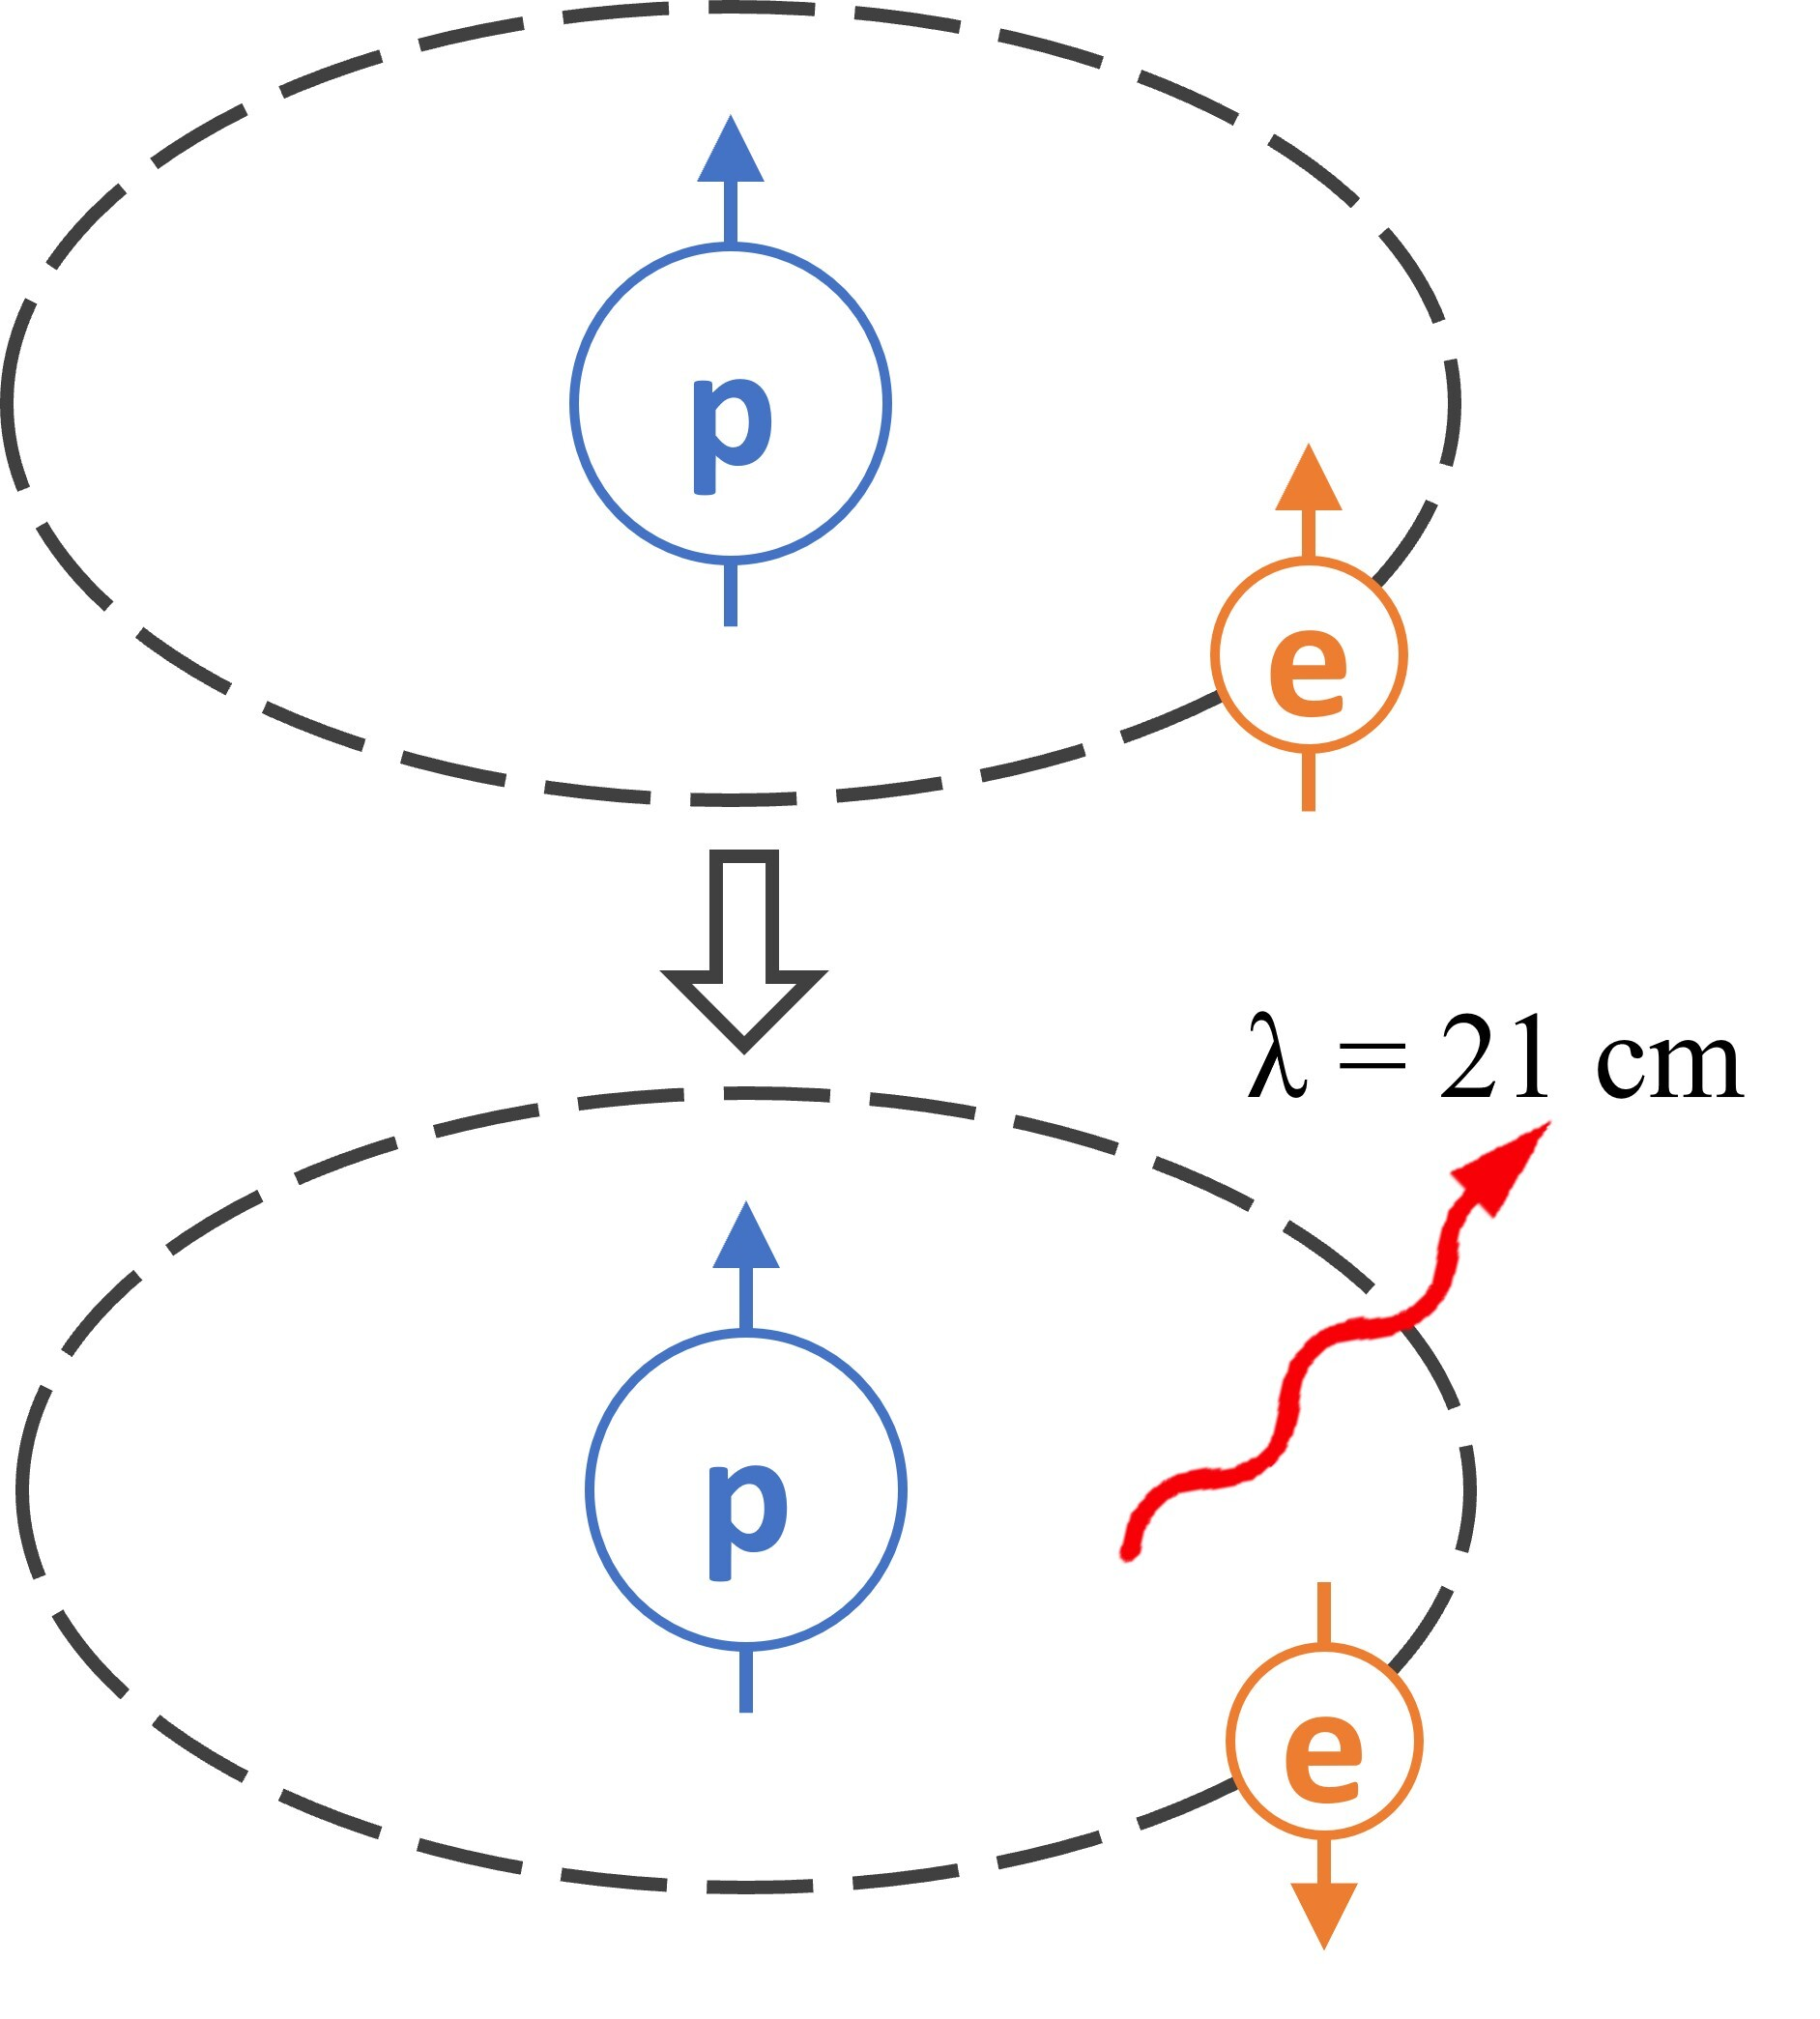
\includegraphics[scale =0.4]{spinflip.jpg}
\caption[Spin-flip Transition of Neutral Hydrogen]{A basic depiction of the spin-flip transition on the ground energy state of the neutral hydrogen. The upper and lower plots demonstrate the classical cartoons of the triplet and singlet states. The energy difference associated with this transition is $\Delta E = 5.9 \times 10 ^{-6}eV$ \cite{21century}. Figure from Kit Gerodias \cite{kit_thesis}.}
\label{fig:spinflip}
\end{figure}

Given that the \gls{cmb} encompasses photons with the wavelength of $21cm$, hydrogen atoms are able to engage in interactions with the \gls{cmb}. As a consequence of this interaction, the brightness temperature of the $21cm$ line experiences an alteration\footnote{This interaction will be discussed in detail in Chapter \ref{chap:global21cm} as the coupling of the spin temperature $T_s$ with the kinetic temperature of the gas $T_k$.}. \hl{This influence can be detected using precise radio telescopes over the frequency range of approximately 30 to 200 $MHz$ (due to the redshifting of $21cm$ photons)}. \cite{low_frequency}. These observations are capable of giving us valuable information about the distribution of neutral hydrogen and the evolution of cosmic structure over time\cite{low_frequency}.\par

\subsection{Physical Principles of The 21cm Spectral Line}
The $21cm$ signal is a result of interaction between the \gls{cmb} and the matter along its way. The characteristics of the signal depend on the radiative transfer along the line of sight. To find the brightness temperature of the $21cm$ line, we start with the basic \gls{rte} for the specific intensity $I_{\nu}$:
\begin{equation}
    \frac{dI_\nu}{ds} = - \alpha_\nu + j_\nu ,
    \label{eq:RT}
\end{equation}
Where $\alpha_\nu$ and $j_\nu$ are absorption and emission coefficients, respectively. This equation is written under the assumption of zero scattering \cite{21century, low_frequency}. \par
We relate the $I_\nu$ to temperature by the assumption of working in Rayleigh-Jeans limit, which gives: $I_\nu = 2k_B T \nu^2 /c^2$. Moreover, the optical depth along the line of sight is defined as $\int \alpha_\nu \left(s\right) ds$, where $ds$ is a path length. Now, we may rewrite equation \ref{eq:RT} \hl{to find the observed brightness temperature $T^{obs}_b$ at a frequency $\nu$ along the line of sight from a background radio source of brightness temperature $T_R$. This radiation passes through a cloud with the optical depth $\tau_\nu$, and uniform excitation temperature $T_{ex}$} \cite{21century, low_frequency}:
\begin{equation}
    T^{obs}_b = T_{ex} \left(1-e^{-\tau_\nu} \right) + T_R \left (\nu \right) e ^{-\tau_\nu}
\end{equation}
For $21cm$ applications, the excitation temperature is referred to as spin temperature $T_S$. It is defined based on the population (number densities) of hydrogen atoms in the triplet ($n_0$) and singlet state ($n_1$) \cite{21century, low_frequency} \footnote{Refer to figure \ref{fig:spinflip} for the definition of hydrogen hyperfine singlet and triplet state.}.
\begin{gather}
    \frac{n_1}{n_0} = \frac{g_1}{g_0} e ^ {-\frac{T_*}{T_S}}\\
    g_0 =1, g_1 =3\\
     T_* \equiv \frac{E_{10}}{K_B} = \frac {hc}{k\lambda_{21cm}} = 0.068 K
\end{gather}
$g_0$ and $g_1$ are the statistical degeneracy factors. The deviation of the spin temperature from the background temperature is the key to the detectability of $21cm$ signal.\par
\begin{comment}
    \footnote{Although it is possible to choose a radio-loud point source as the background template, however since the order of fluctuations in the \gls{cmb} temperature is insignificant in our study ($\delta T_{CMB} \approx 10 ^{-5}$), the \gls{cmb} is a great candidate as a source of uniform brightness\cite{21century}.}
\end{comment}
According to \cite{21century, low_frequency}, the optical depth of a cloud of hydrogen can be written as:
\begin{gather}
    \tau_\nu=\int \mathrm{d} s\left[1- e^{ -\frac {T_*}{ T_S}}\right] \sigma_0 \phi(v) n_0 ,\\
    n_0 =\frac{n_H}{4},\\
    \sigma_0 \equiv \frac{3c^2 A_{10}}{8\pi \nu^2}
\end{gather}
where $\phi(\nu)$ accounts for the line profile, which is normalized such that $\int \phi \left(\nu\right) =1$. $n_H$ is the hydrogen number density, and the $1/4$ factor is the ratio of hydrogen atoms in the hyperfine triplet state to the total number of atoms. $\sigma_0$ represents the $21cm$ cross-section which is dependent on the spontaneous decay rate of the spin-flip transition $A_{10} = 2.85 \times 10^{-15} s^{-1}$ \cite{21century, low_frequency}. The relatively small value of $A_{10}$ implies the rare occurrence of the transition \cite{kit_thesis}. 

Three competing processes influence the spin temperature: 1) interaction of $21cm$ photons with the radio background (mostly \gls{cmb}), 2) collisions with other particles (a mixture of hydrogen atoms, free electrons, and protons with hydrogen atoms as the leading component), and 3) resonant scattering of \gls{lya} photons that cause a spin-flip transition with the meddling of an intermediate excited state. Therefore, the spin temperature will be expressed using the equilibrium between these mechanisms and their corresponding coefficients \cite{low_frequency,21century}:
\begin{equation}
    T^{-1}_S = \frac{T^{-1}_\gamma + x_\alpha T^{-1}_\alpha + x_c T^{-1}_K}{1 + x_\alpha + x_c}.
\end{equation}
Where $T_\gamma$ is the temperature of the surrounding bath of radio photons ($T_\gamma = T_{CMB}$). $T_K$ is the kinetic temperature of gas, and $T_\alpha$ is the color temperature of the \gls{lya} radiation field (at the \gls{lya} frequency). There is a strong coupling between the $T_\alpha$ and $T_K$ as a result of recoil during the repeated scatterings of \gls{lya} photons. $x_c$ and $x_\alpha$ are the coupling coefficients due to atomic collisions and scattering of \gls{lya} photons, respectively. The spin temperature becomes strongly coupled to the gas temperature when coupling coefficients become dominant: $x_c + x_\alpha \gtrsim 1$. On the other hand, it relaxes to $T_\gamma$ when the coefficients are relatively small: $x_c + x_\alpha << 1$ \cite{21century, low_frequency}. \par
The coupling coefficients $x_c$ and $x_\alpha$ are defined as a function of collisional scattering (spin de-excitation) rate $C_{10}$, and \gls{lya} scattering rate $P_{10}$ or $P_\alpha$ \cite{explore_cosmic_dawn, low_frequency}:
\begin{gather}
    x_c \equiv \frac{C_{10}T_*}{A_{10}T_\gamma}\\
    x_\alpha \equiv \frac{P_{10} T_*}{A_{10}T_\gamma} \label{eq:x_a}
\end{gather}
\subsection{Wouthuysen-Field Coupling}
As previously mentioned, a hydrogen atom in the early universe is able to interact with \gls{cmb} background through photon exchange. However, with the onset of star formation, \gls{cmb} will no longer be the only source of photons for the hydrogen atom to interact with. The newly formed compact objects are capable of generating \gls{uv} photons (e.g.,\gls{lya}) and reheating the \gls{igm}. These photons are injected into the \gls{lya} frequency band by resonant scattering rather than being redshifted from outside of the line. The existence of this second source of the photons increases the coupling probability of the hydrogen-background interaction, further assisting the spin temperature $T_S$ in coupling to $T_K$ \cite{21century, low_frequency}.\par
The process of coupling the spin temperature of neutral hydrogen to the \gls{lya} background is called \textbf{\gls{wf} effect} \cite{barkana2001beginning}\footnote{The \gls{wf} coupling is named after two physicists who independently described the phenomenon in 1952 and 1958: Robert H. Wouthuysen \cite{wouthuysen_original}, and George B. Field \cite{field_original}.}. This process plays a pivotal role in the observability of the global $21cm$ signal by forcing it to deviate from the temperature of the \gls{cmb}. The \gls{lya} coupling coefficient, indicating the strength of \gls{wf} effect, was defined in equation \ref{eq:x_a}. \par

\subsection{Sky-Averaged 21cm Signal}
\label{chap:global21cm,sub:physics,sub:global}
We previously mentioned that the global $21cm$ signal is the average over all the spatial fluctuations of the $21cm$ signal. We study the behavior of this signal in comparison to a roughly uniform source of radio background. Thus, we define the differential brightness temperature of the global $21cm$ signal as the excess brightness temperature (due to emission or absorption) of the global $21cm$ signal with respect to that of the \gls{cmb} background. Therefore,
\begin{equation}
    \delta T_b = T_{S} - T_{\gamma} = T_S - T_{CMB}.
\end{equation}
This differential brightness temperature is found using the following expression \cite{low_frequency}:
\begin{equation}
    \delta T_b \approx 27 \left(1- \bar{x}_i\right) \left(\frac{\Omega_{b, 0}h^2}{0.023}\right) \left( \frac{0.15}{\Omega_{m, 0}h^2} \frac{1+z}{10}\right)^{1/2}\left(1-\frac{T_\gamma}{T_S}\right)
    \label{eq:global_curve}
\end{equation}
Where $x_i$ is the ionization fraction, and $h$ is the dimensionless Hubble constant. $\Omega_{b, 0}$ and $\Omega_{m, 0}$ are the ratio of the current energy density of baryonic and total matter with respect to the critical energy density of the universe.\par
To further investigate the evolution of the global $21cm$ through the thermal history of the universe and the physical mechanisms behind the fluctuations, we split the early universe era into different redshift regions\footnote{It is crucial to mention that there is still considerable uncertainty in the exact values of the redshift bounds and the sequence of events due to our highly limited knowledge on the characteristics and effects of early sources. This uncertainty is such significant that there might even be an overlap between these discussed regions \cite{21century}.}:\par
\begin{itemize}
\item $200 \lesssim z \lesssim 1100$ (Dark Ages): The universe is filled with high-density gas and the residual free electrons from the recombination. Compton scattering maintains the thermal coupling of gas to \gls{cmb} ($T_K = T_\gamma$). Due to high density, the collisional coupling is dominant, forcing the spin temperature to the kinetic temperature of the gas ($T_S = T_K$). 
Therefore, the differential brightness temperature of the $21cm$ signal is zero during this redshift regime ($T_S = T_\gamma$)\cite{21century}.\par

\item $40 \lesssim z \lesssim 200$ (Dark Ages): Baryonic matter experiences thermal decoupling from the \gls{cmb}, making it possible for the non-relativistic gas to cool adiabatically with the expansion of the universe \cite{21century}. The temperature of the gas and \gls{cmb} both drop as a function of redshift with the rate of $T\propto (1+z)^{2}$ and $T\propto (1+z)$, respectively. This rate discrepancy leaves the gas cooler than radiation while stopping heat exchange between these two components. Therefore, the gas spin temperate decouples from that of the \gls{cmb}. Since collisional coupling is still dominant, the spin temperature remains coupled to the gas kinetic temperature ($T_S = T_K$). Consequently, the $21cm$ differential brightness temperature becomes negative (absorption) in this redshift region \cite{map_universe, 21century}.\par

\item $40 \lesssim z \lesssim 80$: As the density keeps dropping through the expansion, the influence of collisional couplings becomes less significant, causing the spin temperature to again couple with the \gls{cmb} temperature ($T_S \rightarrow T_\gamma$). Thus, the $21cm$ differential brightness temperature goes back to zero again \cite{map_universe}. The first blue regions in the upper panel of figure \ref{fig:global_signal_pritchard_loeb} and the corresponding absorption trough in the lower panel depict the above-mentioned process \cite{map_universe, 21century}.\par

The second trough in the lower panel of Figure \ref{fig:global_signal_pritchard_loeb} emerged through the formation of the first structures.

\item $z_\alpha \lesssim z \lesssim z_*$: As large halos begin to collapse and form first stars and galaxies, they generate X-ray emission. These photons are capable of heating their surrounding gas. On the other hand, two mechanisms create \gls{lya} photons: 1) Continuous redshifting of background radiation to the \gls{lya} wavelength, and 2) Ionization and deexcitation of \gls{igm} gas. As a result, a \gls{lya} background is formed. Since the emissivity required for the coupling of $T_S$ to \gls{lya} (\gls{wf} coupling) is less than that needed for maintaining the coupling of $T_S$ to $T_\gamma$, the spin temperature tends to couple to $T_k$ \footnote{\hl{Emissivity is a quantitative measure of how efficiently an object emits electromagnetic radiation. In this case, the spin temperature could either maintain its coupling to $T_\gamma$ or couple to the gas kinetic temperature.} The first scenario is disfavored as the radiation heating needs to be very efficient to keep the spin temperature to that of the \gls{cmb}. However, the structure formation has just started, and there are not yet enough X-ray sources to provide the required heating. Thus, the spin temperature varies according to the second option, which is coupling to $T_S$. In other words, the \gls{lya} coupling coefficient $x_\alpha$ becomes dominant over the coupling coefficient $x_c$. Later in lower redshifts, when the population of X-ray sources increases, the heating becomes more powerful, and the coupling to $T_\gamma$ will be again established.}. Therefore, we will again observe the global $21cm$ signal in absorption (the second trough in the lower panel of Figure \ref{fig:global_signal_pritchard_loeb}) \cite{map_universe, 21century}.\par

\item $z_r \lesssim z \lesssim z_\alpha$ (Reionization): Eventually, the gas is reheated by ionizing X-ray photons from early sources \cite{21century}, and the $21cm$ differential brightness temperature becomes positive. The influence of this reheating mechanism is so strong that the $21cm$ radiation can be observed in emission in this redshift range (red region in the upper panel of figure \ref{fig:global_signal_pritchard_loeb}). From this point on in the thermal history of the universe, we do not expect to see any more $21cm$ radiation from \gls{igm} since the majority of the gas will be ionized by emergent stars, galaxies, and accreting black holes. Therefore, the $21cm$ differential brightness temperature goes to zero (the black region in the upper panel of figure \ref{fig:global_signal_pritchard_loeb}). However, in the regions with higher recombination rates inside galaxies and dark matter halos, the neutral hydrogen is shielded and preserved. Consequently, the 21cm signature originating from inside the galaxies will continue to be emitted \cite{map_universe, 21century}.\par
\end{itemize}

\begin{figure}[h!]
    \centering
    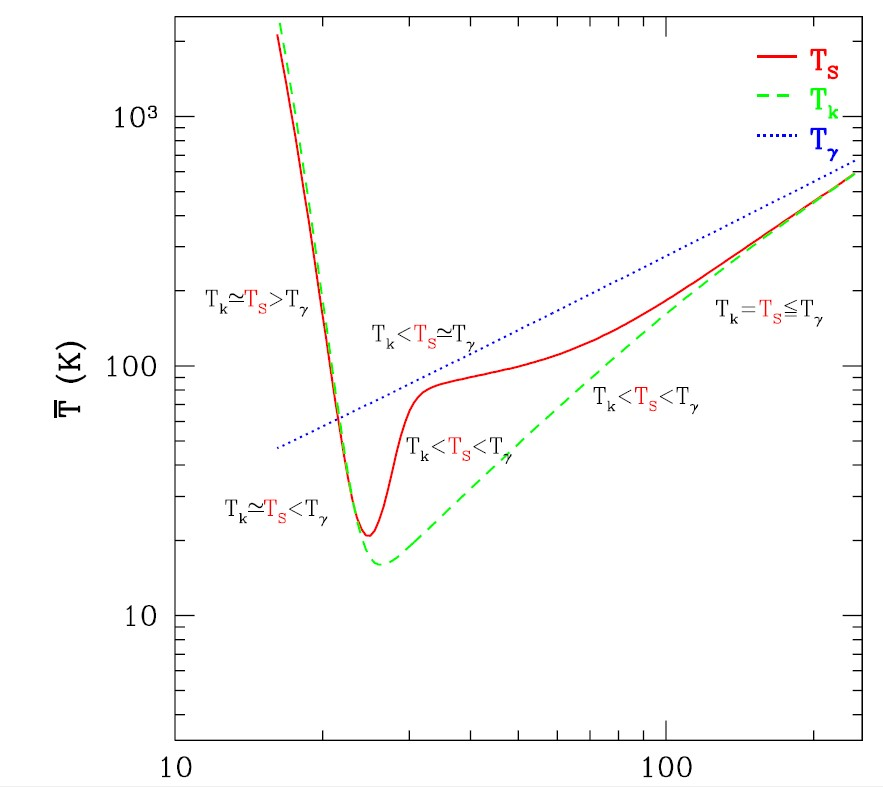
\includegraphics[scale = 0.6]{21cm_curve.jpg}
    \caption[Fluctuation of temperatures involved in the evolution of $21cm$ signal]{Fluctuation of temperatures involved in the evolution of $21cm$ signal. Solid, dotted, and dashed curves represent the spin temperature, \gls{cmb} temperature ($T_\gamma$ or equivalently $T_{CMB}$), and the kinetic temperature of the gas, respectively. Note that this figure displays the spin temperature of $21cm$ signal while figures \ref{fig:global_signal_pritchard_loeb} and \ref{fig:ares_Curve} show the differential brightness temperature. The figure is generated using \gls{21cmfast} \cite{21cmfast_python}.}.
    \label{fig:21cmfast_curve}
\end{figure}

\begin{figure}[h!]
\centering
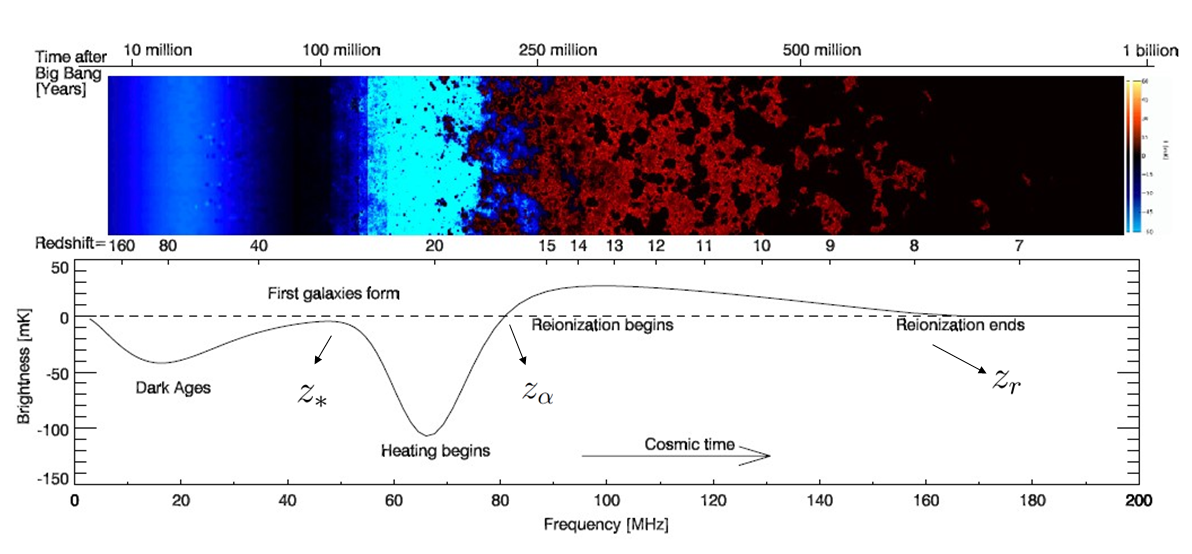
\includegraphics[scale =0.5]{global_signal_pritchard_loeb.png}
\caption[Time evolution of the fluctuations in the $21cm$ differential brightness temperature]{Time evolution of the fluctuations in the $21cm$ differential brightness temperature (solid line). The top panel is a color plot demonstrating fluctuations arising from variations in density. The coloration depicts the two absorption phases of $21cm$ brightness temperature (coupling of $T_S$ to $T_K$, blue regions), emission phase (red regions), and the interval where it disappears completely (coupling of $T_S$ to $T_\gamma$, black region). The lower panel represents the evolution of sky-average (global) $21cm$ signal from the dark ages to the reionization. The frequency range of the absorption and emission regions exactly matches the corresponding regions in the upper panel. The precise details of the shape of this signal are still unidentified due to our lack of knowledge on the nature of early sources\cite{liu2013global}. Figure from Pritchard and Loeb, 2011 \cite{21century}.}
\label{fig:global_signal_pritchard_loeb}
\end{figure}
%-----------------------------------------------------------
\section{Simulating the Global 21cm Signal}
With the current advancements in radio telescope instrumentation, we have entered a data-driven era in $21cm$ cosmology, empowering us to constrain the properties of astrophysical sources responsible for generating this signal. Nevertheless, extracting astrophysical insights from the collected data is a complex task that necessitates the fast and efficient generation of theoretical templates spanning over the parameter space \cite{emulate_21cm}. \par
To reach this purpose, fully hydrodynamic simulations of the 3-dimensional evolution of the $21cm$ signal have been adapted \cite{hydrodynamic_sim}. However, these simulations are computationally expensive, and this restriction will considerably decrease our ability to search the parameters space \cite{ares2014jordan}. 
Semi-analytical methods are the proposed state-of-the-art solutions employing a middle-ground approach between these simulations and fully analytical studies. The results of these semi-analytical calculations are in remarkable agreement with corresponding hydrodynamic simulations while consuming a significantly lower amount of run-time \cite{semi_analytic_1, semi_analytic_2, semi_analytic_3, semi_analytic_4, semi-analytic_5}. \par
\hl{On top of these simulators, some studies have proposed the use of emulators} \cite{emulate_21cm, emulate_21cm_2, emulate_21cm_3}. \hl{These statistical models are trained using the output data of simulators. They "emulate" the behavior of simulators of global $21cm$ signal by learning the complex relationships between input parameters and the corresponding output. Emulators essentially create a fast and approximate surrogate model of the simulator, which can be used to predict the outcome for new input parameter values. While emulators are much faster than running full simulations and allow rapid exploration of parameter space, they are inherently approximations of the underlying physics. Thus, they may not capture all the fine details of the system's behavior.}\par
In this section, we introduce two powerful tools capable of simulating the theoretical $21cm$ curves over a wide range of astrophysical and cosmological parameters. The first one is \gls{21cmfast} \cite{21cmfast_c, 21cmfast_python}, which is a popular tool to simulate the spatial fluctuations of $21cm$ signal. It is also capable of generating the global curve by averaging over all the signals in different directions. The other one is \gls{ares}, which calculates the global curve directly by solving the cosmological \gls{rte} \cite{ares2014jordan}. The main difference between these two comes from the fact that they use different parameterizations of the $21cm$ theory as the basis of their simulations. For global $21cm$ applications, the use of \gls{ares} is preferred over \gls{21cmfast} based on its direct approach for generating the $21cm$ curve. \par

\subsection{21 Centimeter Fast Approximate Signal Toolbox (21cmFAST)}
\gls{21cmfast} is a Python-integrated C package designed to produce 3D cosmological realizations of physical fields playing a role in the early universe. It is based on a semi-numerical approach combining the excursion set formalism with perturbation theory. \gls{21cmfast} is capable of simulating the 3D realizations of density, peculiar velocity, halo, ionization, spin temperature fields, $21cm$, and ionizing flux fields \cite{21cmfast_c, 21cmfast_python, 21cmfast_documentation, 21cmfast_github}.\par
As mentioned above, the original simulation was developed as a C code. Later, in 2020, the equivalent Python package was introduced as the third version of \gls{21cmfast}. The core C code is a high-performance script aiming to identify regions of ionized hydrogen in a complex cosmological density field based on excursion set formalism. The evolution of the field is analyzed using first- or second-order Lagrangian perturbation theory. Taking this approach will result in revealing the history of thermal and ionization states of IGM, alongside X-ray, and \gls{uv} radiation fields, derived from galaxy models \cite{21cmfast_c}. \par
An example of a global curve generated using \gls{21cmfast} is shown in \ref{fig:21cmfast_curve}.
\subsection{The Accelerated Reionization Era Simulations (ARES)}
\gls{ares} is a Python package for generating global $21cm$ curves \cite{ares2014jordan, ares_documentation, ares_github}. Alongside this applications, it can be used for stand-alone non-equilibrium chemistry solver, global radiation background calculator,  galaxy semi-analytic modeling \cite{jordan_galaxy_1, jordan_galaxy_2, jordan_galaxy_3}, PopIII star modeling \cite{jordan_star}, 1D radiative transfer, and \gls{sed} optimization \cite{jordan_SED}.\par
\gls{ares} draws the globally-averaged $21cm$ curve through the numerical calculation of differential brightness temperature $\delta T_b$ (equation \ref{eq:global_curve}). This approach necessitates the evolution of the spin temperature $T_S$, which itself is dependent on coupling coefficients $x_\alpha$ and $x_c$. The collisional coupling coefficient $x_c$ is found using the tabulated values in \cite{ares_collision_coeff}, and the \gls{lya} coupling coefficient is calculated from equation \ref{eq:x_a}. By ignoring detailed line profile effects, this expression can be written in the following form as a function of angle-averaged $Ly\alpha$ back-ground intensity $\widehat{J}_\alpha$, which determines the strength of Wouthuysen-Field coupling \cite{ares2014jordan, ares_lya_coeff_1, ares_lya_coeff_2, ares_lya_coeff_3}:  
\begin{equation}
    x_\alpha = 1.81 \times 10^{11} \frac{\widehat{J}_\alpha}{1+z}
    \label{eq:x_a,j}
\end{equation}
Where $\widehat{J}_\alpha$  is a specification of the general definition of angle-averaged back-ground intensity as a function of co-moving volume density emissivity \cite{ares2014jordan}:
\begin{equation}
    \widehat{J}_\nu (z)=\frac{c}{4 \pi}(1+z)^2 \int_z^{z_{\mathrm{f}}} \frac{\hat{\epsilon}_{\nu^{\prime}}\left(z^{\prime}\right)}{H\left(z^{\prime}\right)} \mathrm{e}^{-\bar{\tau}_\nu} \mathrm{~d} z^{\prime}
    \footnote{In this expression the $\widehat{J}_v(z)$ and $\hat{\epsilon}_{\nu^{\prime}}$  are in units of photon number density:
    $\left[\hat{J}_v\right]=\mathrm{s}^{-1} \mathrm{~cm}^{-2} \mathrm{~Hz}^{-1} \mathrm{sr}^{-1}$,
    $\left[\hat{\epsilon}_v\right]=\mathrm{s}^{-1} \mathrm{~Hz}^{-1} \mathrm{cMpc}^{-3}$.} 
\end{equation}  
Numerical evaluation of this expression is generally computationally heavy, mostly due to the optical depth ($\tau_\nu$) term. A clever solution is to tabulate the optical depth values on an arbitrary number of redshift points in look-up tables. This approach avoids the extensive calculation of this term on each run. However, the accuracy of this method is dependent on the number of chosen redshift points in the look-up table, and undersampling might result in large deviations in background radiation intensity.\par
In summary, \gls{ares} simulates the behavior of \ref{eq:global_curve} as a function redshift and portray the global $21cm$ signal. A typical \gls{ares}-generated curve is presented in \ref{fig:ares_Curve}. \par
\begin{figure}[h!]
    \centering
    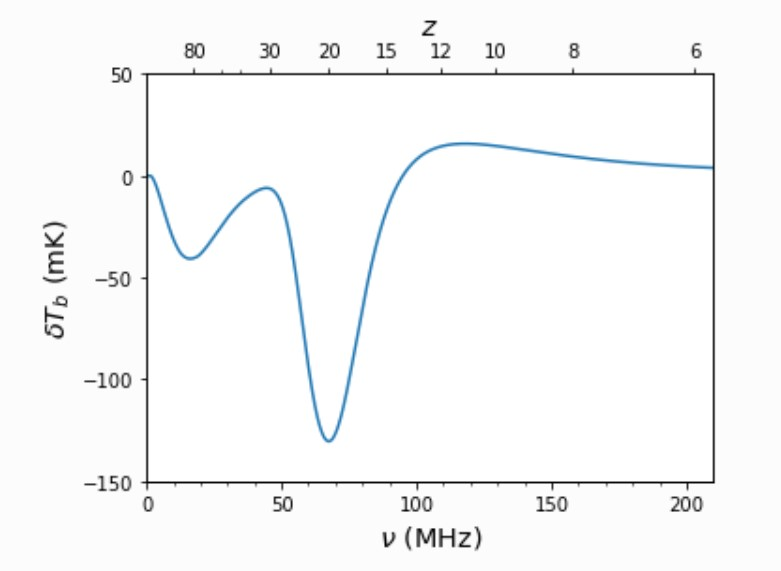
\includegraphics[scale =0.8]{ares_curve.jpg}
    \caption[Typical global $21cm$ curve generated using \gls{ares}]{An example of a global $21cm$ signal generated using \gls{ares}, illustrating the evolution of the brightness temperature of $21cm$ line against the background radio sources as a function of frequency/redshift. The fluctuations discussed in section \ref{chap:global21cm,sub:physics,sub:global} are perfectly demonstrated in the simulated signal. Note the similarities to corresponding regions in figure \ref{fig:global_signal_pritchard_loeb}. Figure from Jordan Mirocha in the ARES documentation \cite{ares_documentation}.}
    \label{fig:ares_Curve}
\end{figure}
%------------------------------------------------------------
\section{Signature of Non-Standard Physics}
\label{chap:global21cm,sub:non_standard}
%add the effects of primordial magnetic fields
The physics of the $21cm$ signal indicates that if the \gls{igm} ionization state is close to neutral and the coupling is saturated, the brightness temperature of this line is strongly dependent on the temperature fluctuations of the \gls{igm}. Therefore, any physical process involving heat exchange with the \gls{igm} is expected to print their signature on the $21cm$ global signal \cite{21century}. Many proposed models of physics beyond the standard model of cosmology and particle physics predict exotic heating of the 
\gls{igm} \cite{21century}, Therefore, we dedicate this section to the investigation of these effects. The exact calculation of these fluctuations on the $21cm$ signal will determine the ability of upcoming observational data to detect these effects.\par
Among these beyond standard models, different dark matter candidates play a pivotal role. For example, it is expected that decaying or annihilating dark matter and evaporation of primordial black holes can inject energy into the \gls{igm} and lead to a stronger brightness temperature of 21cm signal through the \gls{eor}. Therefore, we might be able to constrain these theories by observing their features on the global $21cm$ signal \cite{primordial_bh, new_physics_thesis, primordial_bh_binary, 21limit_dm_bh, bound_dm} or even rule out some of these candidates \cite{rule_out}.\par
Another significant effect comes from the interactions associated with cosmic strings. The non-linear gravitational influence of cosmic string wakes or the decay of cosmic string cups has the ability to alter the brightness temperature of $21cm$ signal \cite{WF_effect_oscar, cosmic_string_oscar, string_loop_robert}. \par
Moreover, rapidly growing radio-luminous black holes of intermediate mass emit radio signals on their way to becoming supermassive black holes. Thus, they are a type of astrophysical radio source with the ability to enhance the amplitude of the global $21cm$ signal \cite{bh_cosmioc_dawn} \footnote{The author of \cite{bh_cosmioc_dawn} claims that the effect of rapidly growing radio-luminous black holes is a reasonable explanation for the signal reported by \gls{edges}.}. \par
In the remainder of this section, we will focus on two of these distinctive non-standard effects, which attracted the attention of the majority of recent literature related to this area of research.\par

\subsection{Dark Matter (DM)}
%I can add some newer papers to this section, from the new directory in my Zotero library
The majority of the proposed \gls{dm} candidates encompass physical mechanisms capable of affecting the baryon temperature and the ionization state of the \gls{igm}. These features can be employed to reveal the interactions of \gls{dm} with the visible sector. Formerly, \gls{cmb} power spectra were used to investigate these signatures. However, the $21cm$ background can probe energy injection rates approximately above $10^{-24}eV cm^{-3} sec^{-1}$ \footnote{The energy density of the \gls{cmb} is approximately $0.26 eV cm^{-3}$, thus $10^{-24}eV cm^{-3} sec^{-1}$ is equivalent to $3.85 \times 10^{-24} s$ of \gls{cmb} emission.}, which is a much higher sensitivity compared to \gls{cmb} power spectra.\par
Decaying or annihilating \gls{dm} produces a secondary source for high-energy particles which, in fact, can heat and ionize the \gls{igm}, contribute to the \gls{lya} background, and leave an imprint on $21cm$ signal.\par
Among these various candidates, decaying or annihilating \gls{dm} may eject energy into the \gls{igm} through the interaction of \gls{dm} particles with known standard model particles. The primordial black hole can also thermally interact with the \gls{igm} in the process of Hawking evaporation and the associated radiations. These effects may lead to a stronger brightness temperature of $21cm$ signal through EoR.  Therefore, we might be able to constrain the characteristics of these theories by their absorption feature in the global 21cm signal (e.g., the lifetime of sterile neutrinos \cite{sterile_neutrino}) \cite{primordial_bh, new_physics_thesis, primordial_bh_binary, 21limit_dm_bh, bound_dm} or even rule out some of the possible candidates (e.g., $3 Kev$ warm \gls{dm} \cite{rule_out}). Some studies even go further and suggest that the use of the $21cm$ gradient alongside its brightness temperature is more efficacious for this purpose \cite{DM_anihilation_furlantto, constrain_dm_21, DM_anihilation_1, DM_ionize, dark_cosmology_21, snowmass_dm}.\par

It must be noted that the presence of additional heating during very high redshifts has the potential to elevate $T_k$ along a higher adiabatic path during the era of collisional decoupling. As a result, this diminishes the depth of the absorption trough around $20 \lesssim z \lesssim 20$. Additionally, if \gls{dm} annihilations contribute to \gls{lya} pumping and heating, the observed signal would exhibit a smoother progression throughout the absorption epoch. A roughly similar process takes place in other extreme astrophysical models with enhanced production of hard X-rays. This degeneracy is an issue in distinguishing the signature of annihilating \gls{dm} in the global $21cm$ signal. However, the spatial distribution of these two heating sources is different, making it possible to differentiate them \cite{dark_nature_21}. \par

Moreover, it has been proved that particle \gls{dm} scenarios featuring a suppressed power spectrum of an astrophysical parameter delay the process of star formation. Since the generation of global $21cm$ signal is dependent on the \gls{uv} radiation of first stars, the corresponding absorption through will occur later than expected. This consequence is stronger in non-cold \gls{dm} models, and their absorption signal models are consistently shifted towards smaller redshifts compared to \gls{cdm}. Therefore, The amount by which the signal is delayed can be used to test non-cold \gls{dm} models  \cite{noncold_dm_21, first_star_impact, dm_timing}.\par 

\begin{figure}[h!]
    \centering
    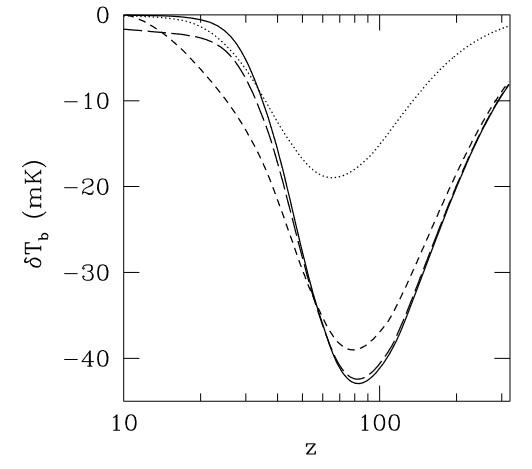
\includegraphics{21cm_dm.jpg}
    \caption[Effect of different \gls{dm} models on the global $21cm$ differential brightness temperature curve]{Effect of different \gls{dm} models on the global $21cm$ differential brightness temperature curve. The solid line shows $\delta T_b$ without decaying/annihilating \gls{dm}, while the long dashed, short dashed, and dotted lines refer to $\delta T_b$ with $25keV$ sterile neutrino decaying \gls{wdm}, $10 MeV$ decaying \gls{ldm} and $10MeV$ annihilating \gls{ldm}, respectively. Figure from \cite{constrain_dm_21}.}
    \label{fig:enter-label}
\end{figure}



\subsection{Cosmic Strings}
 Cosmic strings are hypothetical one-dimensional topological defects in space-time that are predicted as the solution of the field equation in many theories beyond the standard model of particle physics. They are thought to be formed during phase transitions in the early universe \cite{bryce_thesis, constrain_superconduct}.
 It is expected that cosmic strings leave a distinguished signature on the $21cm$ signal in the form of wedge-shaped regions of extra emission or absorption, depending on the value of string tension $G\mu$. The capability of $21cm$ experiments in accessing higher redshift regions (compared to optical large-scale structure surveys) makes them a perfect candidate to search for the effects of cosmic strings  \cite{cosmic_string_brandenberger, structure_cosmic_string}.\par
Two key types of cosmic strings are cosmic string loops and long strings. Long strings refer to the straight or curved sections of cosmic strings that extend over cosmic scales. These strings can be indefinitely long, potentially stretching across vast regions of the universe. Long strings are generally stable and do not decay over time. On the other hand, A cosmic string loop is a closed loop configuration of cosmic string that forms when the string self-intersects or undergoes a reconnection event. These loops are typically much smaller than the cosmic strings themselves and can have a variety of sizes. Cosmic string loops are dynamic structures that can oscillate, radiate gravitational waves, and eventually decay through various processes \cite{cosmic_strings_book}.  \par

Long moving strings make wake regions in space-time. The presence of wakes can lead to the formation of overdense regions, to the point that the baryon density becomes twice that of the cosmic gas. Therefore, the column length line profile of $21cm$ differs from that of the surrounding \gls{igm}, which itself results in a stronger coupling of $T_S$ to $T_K$ in this region. In other words, the \gls{wf} coupling is stronger in the presence of cosmic strings \footnote{Cosmic strings are also expected to speed up the process of reionization due to their early generation of non-linear overdensities\cite{corre_21cm_cmb}.}\cite{cosmic_string_oscar}. With the assumption that X-ray heating is not significant in the \gls{igm}, the brightness temperature of the $21cm$ signal will be at least two times more negative when the effects of cosmic string wakes are included. \par
For string tensions $G\mu \gtrsim 3\times 10^ {-8}$, the signature of the effect of cosmic string wakes becomes larger than noise \cite{WF_effect_oscar}. The signature is also more evident in lower redshifts since string wake width increases as a function of time \cite{cosmic_string_brandenberger}. For small string tensions ($G\mu< 10 ^{-7}$), wake-induced shock heating is not expected. Consequently, the temperature of the gas inside the wake and the \gls{igm} are approximately equal \cite{cosmic_string_oscar}. On the other hand, the shock-heated cosmic string scenario yields an even stronger \gls{wf} coupling (and hence a stronger $21cm$ brightness temperature with a larger amplitude), but the effect from a diffuse wake is extended over a wider redshift interval \cite{oscar_robert_shock, WF_effect_oscar, cosmic_string_oscar}. By calculating the contribution of cosmic string network rather than a single string wake, it was found that the amplitude of the global $21cm$ signal will be enhanced between 10\% to a factor of 2 for string tension in the range of $10^{-8}\lesssim G\mu\lesssim10^{-7}$  \cite{cosmic_string_oscar}.\par

Cosmic string loops are also expected to imprint a roughly elliptical region in redshift with an extra $21cm$ emission \cite{string_loop_robert}.
It is also viable to study the relevant features in the power spectrum of the $21cm$ signal. Calculations prove that the cosmic string $21cm$ power spectrum turns over at smaller scales compared to the inflationary adiabatic $21cm$ power spectrum \cite{super_string}. Overall, since non-Gaussianities in the distribution of strings (that result in a clearer signature) are only visible in position space, they appear to be a superior choice for such studies \cite{cosmic_string_brandenberger}.\par

Another idea is to study this effect in the cross-correlation of $21cm$ radiation, and \gls{cmb} since their existence will simultaneously fluctuate both signals. The cross-correlation observation of these signatures is more reliable compared to individual signals and can be considered evidence of new physics. Unfortunately, the \gls{cmb}-$21cm$ cross-correlation signal might be overwhelmed by sky temperature noise for observationally allowed cosmic string wakes \cite{corre_21cm_cmb}.

In some models of strings, strings carry conserved electromagnetic currents. Thus, they are superconducting \cite{constrain_superconduct}. Some studies have computed the contribution of electromagnetic radiation of annihilating super-conducting cosmic strings to the radio background and derived constraints on the parameter space of superconducting cosmic strings \cite{constrain_superconduct, constrain_spectral_bryce, massive_BH}. By including the effects of these strings to the standard theory, the second absorption trough of the global $21cm$ curve ($z=20$) corresponds to the trough reported by \gls{edges} for string tension of $G\mu = 10 ^{-10}$. However, the slope on the low redshift end tends to be smoother than that of \gls{edges} data. The corresponding string tension is the same order of magnitude as the upper bound reported by pulsar timing array measurements \cite{cosmic_string_jordan_robert, pulsar_timing}. The results of this study are shown in figure \ref{fig:21cm_cosmic_string}.\par
Another possibility is to investigate the effect of decay of cosmic string cusps (ordinary string loops \cite{massive_BH}) on the global $21cm$ signal. As calculated by \cite{robert_cusps}, the depth of the absorption through will only be modified by one part in $10^4$ considering this scenario, which is too weak to constrain the parameter space of the proposed theory.\par

\begin{figure}[h!]
    \centering
    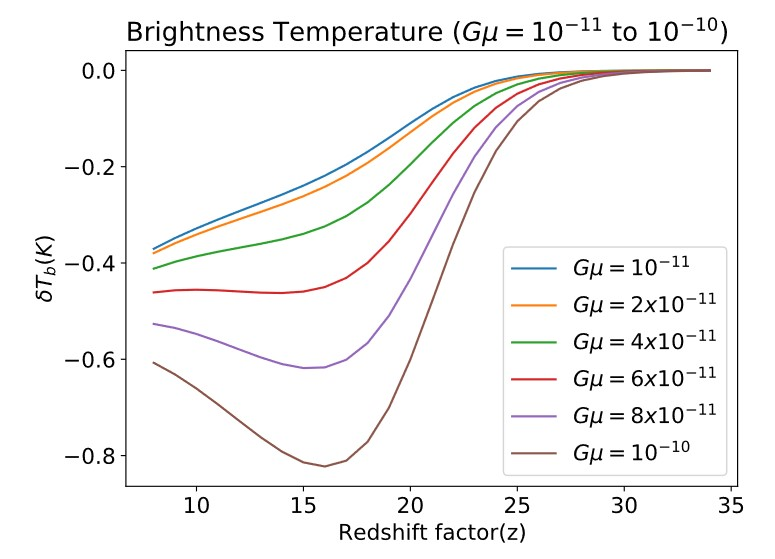
\includegraphics[scale = 0.8]{21cm_cosmic_string.jpg}
    \caption[The global $21cm$ for different values of superconducting cosmic string tension]{The differential brightness temperature of $21cm$ signal as a function of redshift for six different values of superconducting cosmic string tension. The electromagnetic radiation emitted from the decay of superconducting cosmic strings modifies the radio background based on the value of string tension. \hl{This alteration significantly affects the depth of the global $21cm$ absorption trough} (note the difference with Figures \ref{fig:global_signal_pritchard_loeb} and \ref{fig:ares_Curve}). For the critical tension value of $G\mu = 10 ^{-10}$, the trough approaches that of \gls{edges} data. Figure from \cite{cosmic_string_jordan_robert}.}
    \label{fig:21cm_cosmic_string}
\end{figure}

%##############################################################
\chapter{Observations of the Global 21cm Signal}
\label{chap:observations}
The global $21cm$ signal acts as an astrophysical probe to study the early universe. However, as promising as the theory sounds, the actual detection is not a straightforward task. In fact, the challenges of this specific observation are significantly more than those of \gls{cmb} or tomographic $21cm$ maps. 
This radiation possesses the ability to penetrate through dust and Earth's atmosphere, making it possible to be detected with ground-based observations. Since this signal is associated with the dark ages in the redshift range of $30 \lesssim z \lesssim 1100$, corresponding to the frequency range of $1.3 MHz\lesssim \nu \lesssim 50 MHz$, the observations are considered as low-frequency radio experiments \cite{thesis_pamela, thesis_moso}.
Global $21cm$ observations do not require high spatial sensitivity; therefore, they can be carried out by single dipole antennas rather than large interferometric arrays used in measuring fluctuations of $21cm$ signal \cite{thesis_shedding} \footnote{There exist some exceptions to this statement, such as \gls{leda} experiment, which will be discussed in the next section.}.\par
In this chapter, we first discuss the obstacles to the detection of the global $21cm$ signal. Then, we introduce a number of experiments specifically designed to observe this emission. Finally, we will revisit the claimed observation by the \gls{edges} group, the corresponding interpretation, and its contrast with \gls{saras} observations \cite{saras_curse_edges}.
%-------------------------------------------------------------------------------------------------------
\section{Challenges of Global 21cm Observations}
Detection of the global $21cm$ signal is one of the major challenges of radio cosmology. The complexity of this assignment is a result of the bright foregrounds in low frequencies. Unlike CMB observations which have minor foregrounds in the desired frequency range, the intensity of global $21cm$ foregrounds is typically 4 to 5 orders of magnitude stronger than the desired cosmological signal and therefore dominates the data entirely. The mitigation process is also complicated as both the foreground contamination and the theoretical signal are smooth as a function of frequency, making it difficult to use foreground subtraction techniques formerly used for spatial fluctuation maps\cite{liu2013global, thesis_moso, thesis_shedding}.\par
To overcome these concerns, the first step is to avoid noise sources. Several precautions in terms of timing and location of observations are taken to ensure the data is being collected with the least possible foregrounds. The remainder of the noise shall be removed by data analysis techniques through the construction of a practical noise model. To ensure accurate foreground mitigation, this noise model should closely mimic the characteristics of the noise sources. Three major sources contribute to the noise associated with low-frequency observations in the frequency range favored by global $21cm$ experiments: cosmic foregrounds (galactic and extra-galactic), ionospheric effects, and human-generated \gls{rfi} \cite{thesis_pamela, thesis_shedding, book_21cm}. This section is dedicated to the study of these sources and their associated behaviors\par

\subsection{Astronomical Foreground Emission}
The main obstacle of global $21cm$ observations is a consequence of astronomical foreground emission, which is particularly stronger at lower frequencies. The foreground consists of two main types: galactic and extra-galactic. The galactic case comes from the diffuse synchrotron and free-free emission from the Milky Way (such as thermal bremsstrahlung of free electrons). The contribution of synchrotron radiation is approximately two to three orders of magnitude larger than free-free emission\footnote{The exact ratio depends highly on the frequency of interest.}. Moreover, the synchrotron emission is generally stronger along the galactic plane of the Milky Way \cite{thesis_shedding, thesis_pamela, pritchard_mcmc, reionization_old}.
In the extra-galactic case, the emission is a cause of the \gls{agn}, star-forming galaxies, quasars, and other radio-loud sources \cite{book_21cm}. Furthermore, the same radiation process described for Milky Way applies to other galaxies as well. Overall, the contribution of galactic sources is larger than extra-galactic ones \cite{pritchard_mcmc, reionization_old}.\par

Several methods have been proposed to remove the astronomical foregrounds from the highly contaminated raw data provided by global $21cm$ experiments. Mapping of Galactic foregrounds, statistical techniques, including principal component analysis \cite{principal_component}, filtering \cite{filtering}, and machine learning algorithms \cite{removal_deep_learning, signal_reconstruction, signal_extraction, extract_foreground, pritchard_mcmc} appears to be the most promising\cite{thesis_pamela}.\par

\subsection{Ionospheric Effects}
The ionosphere is a layer in the Earth's upper atmosphere ($50km \lesssim h \lesssim 1000 km$). When high-energy particles or sunlight (which includes X-ray and \gls{uv} radiation) pass through the atmosphere, the interaction leaves the gas molecules ionized, resulting in the creation of plasma. The generated ions are capable of reflecting or absorbing radio emissions and therefore interfere with other radio signals passing through this layer. This influence is even more severe in low frequencies, overlapping with the frequency range of the dark ages signal. The ionosphere is the primary origin of systematic aberration, restricting our capacity to investigate the low-frequency domain via radio interferometers \cite{thesis_pamela, ionosphere_ultra_low}.\par
The threshold frequency under which the ionosphere scatters absorbs all radio waves and becomes completely opaque is called the \emph{plasma cut-off frequency} \cite{ionosphere_effect_book, thesis_pamela}. This cut-off is a function of electron density in the ionosphere and generally varies between $2-20MHz$. The electron density itself depends on the time of day, season, altitude, and solar activity. This effect is more severe during the summer days and in regions with higher altitudes, forcing the cut-off frequency to higher amounts during these periods. Thus, winter nights in polar locations during the solar minima have a balance of the best accessible features for earth-based low-frequency observations  \cite{thesis_pamela} \footnote{Long winter nights allow ions to have more time to recombine.}.\par
Constructing theoretical models for ionospheric effects is the key to the mitigation of this foreground from data collected by Earth-based low-frequency observations, resulting in the extraction of the original cosmological signal \cite{ionosphere_model, ionosphere_Bayesian}. However, the most effective way to avoid contamination of data with ionospheric influences is to observe from outside of Earth\cite{thesis_shedding}. A few such experiments have been proposed, yet none of them has been implemented \cite{dare_1, dare_2, 21cm_space_interferometer, lunar_orbit_21cm}. \par

\subsection{Radio Frequency Interference (RFI)}
Terrestrial \gls{rfi} is another cause of challenge for low-frequency observations, which comes from both human-generated sources and natural ones. The observation frequency band of 21cm observations overlaps with a portion of those employed by television stations, satellite or aircraft communications, and ground-based radio transmitters. Particularly, \gls{fm} radio broadcasting band ($88-108MHz$ corresponding to $z \approx 12-15$) is a crowded frequency region and interferes with the detection of the cosmological signal \cite{sci-hi_1}. 
Besides human-made \gls{rfi}, ionized meteor shower trails can reflect radio waves and increase the occurrence of \gls{rfi}. They collide with the Earth's atmosphere and ionize the molecules \cite{prizm_thesis}. This effect is more evident in remote locations where radio antennas are installed. Moreover, telescopes themselves may self-generate \gls{rfi} through unshielded electronics \cite{thesis_pamela}. \par
As the first step in the procedure of avoiding and removing the effects of \gls{rfi} from cosmological data, telescopes are deployed in remote radio-quiet locations (e.g., South African Karoo desert \cite{reach_design}, the Western Australian desert \cite{edges}, and sub-Antarctic Marion Island \cite{prizm_2017, prizm_thesis, rfi_1}). Furthermore, major observations are scheduled during low-\gls{rfi} periods (e.g., nights) \cite{leda_design}. A more productive approach is to position them in locations outside of Earth. Some studies propose radio interferometers to be installed on the far side of the Moon \cite{lunar_far_side, global_moon_far_side} to avoid interference from both the ionosphere and human-made \gls{rfi} \cite{thesis_pamela}. \par
%--------------------------------------------------------------------------------------------------------
\section{Global 21cm Experiments}
Several experiments are dedicated to the observation of the $21cm$ signal and its spatial fluctuations, but only a few of them are specifically designed to detect the global $21cm$ signal. As mentioned earlier, this detection is very challenging due to the powerful foregrounds in the desired frequency band of the cosmological signal. The ongoing Global 21 cm experiments are generally composed of wideband antennas connected with a correlation spectrometer. They vary in terms of antenna frequency response and the approach employed for calibration of the systematic instrumental effects \cite{hyperion_1}. Successful detection of global $21cm$ signature is dependant on measurements with the accuracy of order $1:10^5$. Accomplishing this sensitivity requires smart system engineering and tuned electrical performance \cite{hyperion_2}. In this section, we will present a brief review of some of the ongoing global $21cm$ experiments.\par

\subsubsection{Experiment to Detect the Global EoR Signature (EDGES)}
The collaboration between MIT Haystack Observatory and Arizona State University, aiming to detect the global $21cm$, is known as \gls{edges} \cite{edges_website_1, edges_website_2}. Located at the Murchison Radio-astronomy Observatory and Mileura Station in Western Australia, the \gls{edges} group has developed four versions of the instruments in the past decade. Each radiometer is basically a single compact dipole-like antenna alongside a well-calibrated radio receiver. The measurement calibration of the instrument has proven to possess the levels of accuracy needed for 21cm observations \cite{edges_calibration_1, edges_calibration_2}. The early results of this experiment ruled out models of rapid realizations as well as models of early star formation, especially those with little or late X-ray heating \cite{edges_lower_limit, edges_high_band_constrain}. In 2018, the \gls{edges} team reported the first-ever claim of the detection of the global $21cm$ signal \cite{edges}. They found an absorption profile in the global radio spectrum centered at a frequency of 78 MHz ($z\approx 17$) with an amplitude of $500mK$. The depth of the observed trough is more than a factor of two greater than the largest standard theoretical predictions. Moreover, the overall behavior (shape) of the signal is significantly different from the expectation of the \gls{lcdm} model. Currently, the $21cm$ community endeavors to build new radiometers to confirm the \gls{edges} detection or attempt to explain the reported signal through the utilization of non-standard scenarios \cite{dark_ages_space, thesis_shedding, edges_toward_emprical}.\par

\subsubsection{Shaped Antenna measurement of background RAdio Spectrum (SARAS)} 
Initially sited at the Raman Research Institute in India, \gls{saras} is another experiment with the goal of detecting global spectral distortions from redshifted $21cm$ signal during Cosmic Dawn and Reionization. The radiometer utilized a fat-dipole antenna with a frequency-independent beam \cite{saras_1}. Motivated by the advantages of monopole antennas over dipoles in terms of frequency independence, the modified \gls{saras}2 version was a shaped monopole antenna deployed at the radio-quiet Timbaktu Collective in Southern India \cite{saras_2}. \gls{saras}2 eventually provided more promising results compared to the original \gls{saras}1 experiment. The collected data targeting the $110-200 MHz$ frequency band were examined for signatures of cosmological reionization, and soon they rejected the class of cosmological models offering rapid reionization or inefficient primordial gas heating (very cold IGM at the epoch of the Cosmic Dawn, resulting in deep $21cm$ absorption troughs) \cite{saras_2_constrains, saras_2_results}. These findings were inconsistent with the \gls{edges} claimed detection\footnote{This inconsistency will be discussed thoroughly in section \ref{chap:Observations,sub:edges_affair}.}\cite{dark_ages_space, thesis_shedding, saras_curse_edges}.\par
\hl{The design was later progressed in terms of calibration techniques to eliminate errors in the receiver system and avoid unwanted structures from intense foregrounds}. The efforts paved the way for the \gls{saras}3 experiment that is optimized for the $50-100 MHz$ band \cite{saras_3, dark_ages_space}. Later, in 2022, findings of \gls{saras}3 experiment revealed the non-detection of signal reported by \gls{edges} \cite{saras_3_results}.\par
%Moreover, the Indian space agency (ISRO) has granted pre-project funding to the \gls{saras} team to develop a lunar orbiter mission \cite{dark_ages_space}.\par

\subsubsection{Probing Radio Intensity at high-Z from Marion (PRI$^Z$M)}
\gls{prizm} is a recent effort to study the cosmic dawn and dark ages. This experiment is specially designed to collect global $21cm$ data in the frequency range of $50-150MHz$. The distinguishing feature of this experiment is its exceptionally isolated and radio-quiet location on an island in the sub-Antarctic Southern Indian Ocean called \emph{Marion}. This island is approximately 2000km away from the nearest continental land masses and any human-habited regions. With no detected \gls{rfi} contamination in the FM band, Marion is one of the prime locations on Earth for radio observations. The experiment consists of two modified four-square radiometers, operating at center frequencies of 70 and 100 MHz, and a dual-polarization spectrometer back end. The antenna was originally designed for \gls{sci-hi} experiment \cite{sci-hi_1, sci-hi_2} and later modified for \gls{prizm}. After its deployment in Marion in 2017, \gls{prizm} started its science observations. Currently, the collected raw data is being analyzed to extract the cosmological sky-averaged $21cm$ signal \cite{prizm_2017, prizm_thesis}.\par 

\subsubsection{Radio Experiment for the Analysis of Cosmic Hydrogen (REACH)}
The \gls{reach} experiment is another wideband global $21cm$ project led by Cambridge University, covering both the cosmic dawn and the epoch of reionization. The antenna is designed as a seven-pointed blade (hexagonal dipole) with conical log spirals, covering the frequency range of $50-135MHz$ ($7.5 < z < 28$). In the future, multiple antennas (scaled and/or different types) will be added to form a joint confident detection. \gls{reach} phase I was deployed in the \gls{rfi}-quiet Karoo radio astronomy reserve in South Africa in 2022 \cite{reach_z, reach, reach_design}. \par

\subsubsection{Mapper of the IGM Spin Temperature (MIST)}
The \gls{mist} experiment plans to perform measurements of the global radio spectrum within the frequency range of $25-105 MHz$. The deployment took place in different remote locations, such as Axel Heiberg Island in Canadian Arctic. This radiometer uses a blade dipole with two panels. The first two antennas of this project are currently gathering data, and the third is undergoing the construction procedure \cite{mist, mist_presentation, mist_website}.

\subsubsection{Large aperture Experiment to Detect the Dark Ages (LEDA)}
Driven by the constraint of single-antenna experiments of the global $21cm$ signal, \gls{leda} collaboration constructed a single-layer multi-antenna instrument (array of simple dipole antennas) to observe the early universe in $30-85MHz$ band ($16 < z < 34$).
This unique 512-input $100MHz$ correlator is installed in two locations: \gls{lwa} stations at \gls{ovro} (\gls{ovro}-\gls{lwa}) and the National Radio Astronomy Observatory in Socorro, New Mexico (LWA1). 
The \gls{ovro}-\gls{lwa} site consists of 251 stands within a $100m$ radius, which is approximately two times the radius of LWA1. The two stations share the same antenna design and analogue systems, but the digital system is distinct\footnote{\gls{ovro}-\gls{lwa} uses a digital system specially designed for wide-bandwidth cross-correlation.}. The integrated \gls{leda} correlator achieved its first light in August 2013 and has been performing science observations ever since \cite{leda_beam, leda_foreground, leda_1, leda_2, leda_design}.\par

\subsubsection{Hydrogen Probe of the Epoch of REIONization (HYPERION)}
The \gls{hyperion} project is another global $21cm$ experiment that was initially deployed at \gls{ovro}. It is composed of a single-element radio telescope system with a two-channel interferometric/cross-correlation spectrometer. The system architecture consists of an electrically short fat dipole with a frequency-independent antenna beam between $30-120 MHz$. The design was directly inspired by the \gls{saras} experiment, albeit tailored specifically for lower frequencies through scaling.\cite{hyperion_1, hyperion_2, hyperion_3}.\par
%a double octave bandwidth short dipole antenna with
%8 element interferometer,  

\subsubsection{Broadband Instrument for Global HydrOgen ReioNisation Signal (BIGHORNS)}
The \gls{bighorns} is a portable total power radiometer that can be deployed in any remote location without access to electricity. The experiment targets the frequency range of $\approx 50 \text{-} 200 MHz$. The first deployments took place at a few radio-quiet locations in Western Australia (Wondinong Station in April 2014, followed by other deployments in  Muresk and Perth). The initial antenna design was based on an off-the-shelf biconical antenna, which was later replaced with a bespoke conical log spiral antenna \cite{bighorns_1}.
%--------------------------------------------------------------
\section{On The Interpretation of EDGES Data}
\label{chap:Observations,sub:edges_affair}
%If asked, I will add the foreground removal technic of edges in this section!
 In 2018, the \gls{edges} collaboration presented the measurements of an anomalously large and abrupt absorption signal in the radio spectrum, which was in apparent contradiction to the theoretical expectations \cite{edges}. The amplitude of the signal is more than a factor of two greater than the corresponding expected signal from \gls{lcdm} model. Moreover, the shape of the curve does not comply with the smooth transition in the theoretical signal. Figure \ref{fig:edges_data} demonstrates the claimed detection, and its comparison with the \gls{ares} simulated global $21cm$ curve generated using the default values of \gls{ares} for cosmological and astrophysical parameters \cite{ares_documentation}.\par
\begin{figure}[h!]
    \centering
    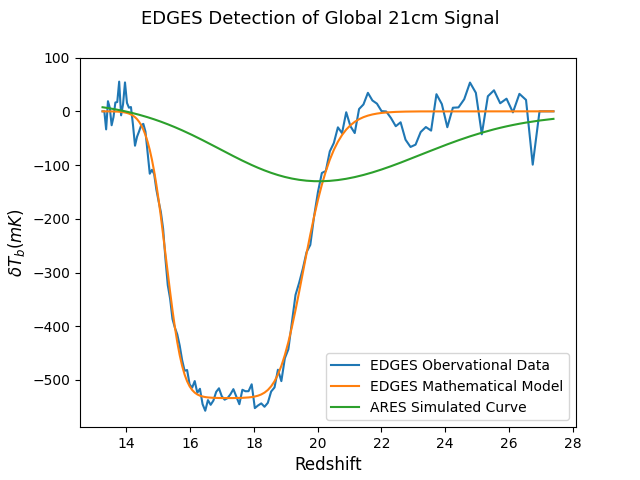
\includegraphics[scale= 0.8]{edges_data.png}
    \caption[Results of \gls{edges} Experiment]{Detection of global $21cm$ signal reported by the \gls{edges} collaboration. The blue curve illustrates the observational data, and the orange curve is the mathematical model (flattened Gaussian) which \gls{edges} group used for the purpose of fitting their data. There is no direct connection between this model and the underlying physics of the global $21cm$ signal. This model is only chosen based on the similarity of its shape to that of the experimental signal. The green curve is an \gls{ares} simulation in the exact redshift range of \gls{edges} data. It is generated using the default values of \gls{ares} for cosmological and astrophysical parameters \cite{ares_documentation}. Note the significant discrepancy in the amplitude and shape of the observational and theoretical curves. Figure generated using data from \cite{edges}.}
    \label{fig:edges_data}
\end{figure}
 
 This observed large amplitude can only be a cause of two scenarios: 1. The gas kinetic temperature is lower than theoretical expectations, 2. There exists some excess radio emission in the background, implying that the temperature of the radio background is hotter than expected in the frequency range corresponding to dark ages and reionization. \par
 The standard cooling mechanism influencing different components of the universe is a result of adiabatic expansion. However, for the gas to be this cold at this redshift, extra cooling mechanisms shall be present at the cosmic dawn to derive the spin temperature to such a low value. Following this idea, many authors have proposed physical mechanisms beyond the standard model of particles and astrophysics to achieve a cooler IGM. \gls{dm}-baryon interactions can be considered as a source of extra cooling through the transmission of thermal energy from baryonic particles of gas to \gls{dm} particles \cite{dm_edges_1, dm_edges_2, dm_edges_3, dm_edges_4, dm_edges_5, dm_edges_6} (refer to \ref{chap:global21cm,sub:non_standard} for a detailed discussion on the influences of various non-standard scenarios on the global $21cm$ signal).\par
 Regarding the background radio emission, it is often assumed that the background radio bath is mainly composed of \gls{cmb}, and subsequent calculations are built upon this approximation. However, the \gls{edges} signal gave rise to the idea that there might be excess radio emission in the cosmic Dawn that increases the spin temperature \cite{excess_radio}. Recent studies revealed that the diffuse radio background from astrophysical origins is unable to explain the discrepancy \cite{excess_radio, thesis_shedding}.\par
 Apart from the inexplicable amplitude, the shape of the reported signal is also a source of concern, as the width of the trough is evidently different from the theoretical expectation. In fact, only astrophysical models based on strong heating of the \gls{igm} are able to justify the width, which is opposite to what is required to obtain large amplitudes. Thus, within the framework of the current formulation of $21cm$ cosmology, the \gls{edges} reported signal includes inner inconsistency \cite{edges_inconsistent_inner, thesis_shedding}.\par
 On top of all these discussions, findings of \gls{saras}2 experiment performed in the same redshift range as \gls{ares} have disfavored models offering a cold \gls{igm}, which is clearly in tension with EDGES results \cite{saras_2_constrains, saras_2_results}. Moreover, the modified version of the experiment, \gls{saras}3, has reported the absence of the aforesaid absorption trough in their investigations. From their point of view, considering the potential sources of systematic errors and instrumental artifacts that could have influenced the observed signal, it is unlikely that the reported trough is a signature of an astrophysical phenomenon \cite{saras_3_results, saras_curse_edges}.\par
%#################################################################
\chapter{Parameter Estimation Methods}
\label{chap:method}
We formerly discussed the physics of global $21cm$ signal and associated observational attempts. We also pointed out the capacity of the global $21cm$ signal to constrain the cosmological and astrophysical parameters and demonstrate the signatures of theories beyond the standard model. However, the details of the process to extract this piece of information from the existing and upcoming observational data are yet to be addressed. \par
The majority of proposed non-standard mechanisms are expected to leave their footprints on the value of physical parameters. Therefore, the urge to perform proper parameter estimation on the corresponding observational data is undeniable. Based on this knowledge, we dedicate this chapter to the construction of a firm computational framework specifically designed for the global $21cm$ parameter estimation. \par
Previous studies have examined various computational algorithms to accomplish this task. The efforts include \gls{mcmc} \cite{pe_mcmc_1, pe_mcmc_2}, \gls{ann} \cite{pe_nn_1}, and even Fisher Matrix approaches \cite{pe_fisher_2}. Sampling algorithms such as \gls{mcmc} are capable of exploring the entire likelihood surface. On the other hand, neural networks are typically employed for problems where comprehensive mapping of the entire likelihood surface becomes excessively complex. \hl{For global 21cm applications, the entire likelihood surface is accessible, thus the use of} \gls{mcmc} method is preferred.\par
We proceed by introducing the main parameter estimation algorithm used in our study, which is a combination of \gls{lm} and \gls{mcmc}. We explain the reason behind utilizing both of these algorithms for this particular fitting challenge and provide a detailed explanation of the procedure to combine them. We also discuss two different tests used to measure the quality of the proposed fit. In chapter \ref{chap:results}, we present the results of applying this fitting method to the observed global $21cm$ signal (\gls{edges}) and its corresponding theoretical model generated by \gls{ares}\footnote{Python Implementation of the analysis of this thesis is publicly available on GitHub under the dedicated repository: 
\href{https://github.com/aryana-haghjoo/My-Project/tree/main/code_final}{https://github.com/aryana-haghjoo/My-Project/tree/main/code\_final}}.\par
%------------------------------------------------------------------
\section{Levenberg-Marquardt (LM)}
\label{chap:method,sub:LM}
The \gls{lm}, also known as the \gls{dls} method, is a fitting algorithm used for non-linear least-squares problems. This iterative algorithm is based on another root-finding method referred to as "Newton's method". \gls{lm} is capable of fitting models with Gaussian-shaped likelihood spaces. However, its abilities are limited when it comes to fitting error bars.\par
In this chapter, we derive the basic analytical definition of this method. We start by defining the matrix form of chi-square. Subsequently, we calculate the second-order derivative of chi-square with respect to the parameters of the model. We will show that this calculation leads to defining the covariance matrix, which forms the basis to generate correlated noise for the \gls{mcmc} algorithm (refer to \ref{chap:method,sub:correlated noise}).\par
\subsection{Covariance Matrix}
\label{chap:method,sub:cov_mat}
A traditional fitting problem is generally defined as trying to find the parameters in a theoretical model which can best explain a set of data and its associated noise. A possible measure for the quality of fit is the value of likelihood. With the assumption of Gaussian noise, the procedure to maximize the likelihood in the presence of noise leads to the minimization of the 
an expression called the "chi-square". The linear algebra notation of the chi-square is
\begin{gather}
    \chi^2 \equiv \left (d-A\left(m\right)\right)^T N^{-1} \left(d-A\left(m\right)\right),
    \label{eq:chi-square matrix}
\end{gather}
Where $d$ is the array containing the data points and $A$ is the model which is dependent on the parameter set m (the dependency can be nonlinear). Thus, $A(m)$ is the representation of the expected value of the data with respect to the theoretical model. $N$ is also defined as the noise matrix, which in general, is non-diagonal. In the case of a diagonal noise matrix, expression \ref{eq:chi-square matrix} takes the form of:
\begin{gather}
    \chi^2 = \sum \frac {\left(x_i - \mu_i\right)^2}{\sigma^2_{i}},
    \label{eq: chi-sqaure simple}
\end{gather}
Where $x_i$ is the observed data, $\mu_i$ is the expected value ($\mu_i=\left<d_i\right>=A_i\left(m\right)$), and $\sigma$ is the error associated with each data point ($N_{i, i} = \sigma^2_{i}$). We continue by calculating the first two derivatives of the above expression, leading to the construction of the gradient descent method.
\begin{gather}
        \frac{d \chi^2}{dm} = - \left(\frac{dA\left(m\right)}{dm}\right)^T N^{-1} (d-A(m)) - \left(d-A\left(m\right)\right)^T N^{-1} \left(\frac{dA(m)}{dm}\right ) 
\end{gather}
We define $A' \equiv\frac{dA(m)}{dm}$, and $r \equiv d - A(m)$. Thus, the above expression takes the form:
\begin{equation}
    \frac{d \chi^2}{dm} = - \left(A'\right)^T N^{-1} r - r^T N^{-1} A'.
    \label{eq:csq_first_deriv}
\end{equation}
Since we know that 
\begin{gather}
    \left(N^{-1}\right)^T = N^{-1}\\
    \left[A' N^{-1} r\right]^T = r^T N^{-1} \left(A'\right)^T,
\end{gather}
substituting in \ref{eq:csq_first_deriv}, we get
\begin{align}
    \frac{d \chi^2}{dm} = -2 \left(A'\right)^T N^{-1} r.
\end{align}
Thus, we can calculate the second derivative:
\begin{align}
    \frac{d^2 \chi^2}{dm^2} = -2 \left(\frac{dA'}{dm}\right)^T N^{-1} r -2 \left(A'\right) ^T N^{-1} \left(-A'\right).
\end{align}
Neglecting the initial term is generally considered safe, as the $r$ component, which represents the difference between the model and data, can have positive or negative values. Consequently, its average approaches zero. Furthermore, our primary objective is to achieve a zero chi-square gradient. Hence, it is acceptable if the curvature is slightly deviated as long as we attain the maximum likelihood. It is worth noting that the purpose of using \gls{lm} is solely to generate a covariance matrix for our \gls{mcmc}. Thus, the generated covariance matrix does not need to be flawless.

Finally, using the above-mentioned logic, we are left with:
\begin{align}
         \frac{d^2 \chi^2}{dm^2} = 2 \left(A'\right)^T N^{-1} A' ,\label{eq:csq_second_deriv}
\end{align}
Which is the definition of the curvature matrix. Our primary focus lies not on this matrix itself but rather on its inverse. The inverse is called the \textbf{Covariance Matrix}. The diagonal elements of this matrix are simply the variance of each parameter ($\sigma_{i, i}$), while the off-diagonal elements represent the covariance, measuring the dependency of a pair of parameters ($\sigma_{i, j}$). In general, we expect the covariance matrix to be semi-positive definite\footnote{A positive definite matrix only possesses positive eigenvalues. However, for a semi-positive definitive matrix, eigenvalues are non-negative.}.\par
%----------------------------------------------------------------------
\subsection{Derivation of the Levenberg-Marquardt Algorithm}
In the \gls{lm} method, on each iteration, the set of parameters m is replaced with $m+\delta m$. To find the $\delta m$, the function $\chi^2 (m +\delta m)$ is approximated by its linearization: 
\begin{gather}
    \chi^2 \left(m\right) = r^T N^{-1} r\\
    \chi^2 \left(m + \delta m\right) =  \chi^2 \left(m\right) + \left(\frac{d \chi^2}{dm}\right) \delta m \label{eq:csq_perturb_deriv}
\end{gather}
Similar to the procedure done in section \ref{chap:method,sub:LM}, we calculate the derivative of \ref{eq:csq_perturb_deriv}:
\begin{gather}
    \frac{d \chi^2 \left(m +\delta m\right)}{dm} = \frac{d}{dm} \left(\chi^2\right) + \frac{d}{dm} \left(\frac{d\chi^2}{dm} \delta m\right)
\end{gather}
We already derived the expression for the first order derivative of chi-square in \ref{eq:csq_first_deriv}. Therefore:
\begin{gather}
   \frac{d \chi^2 \left(m +\delta m\right)}{dm} =  -2 \left(A'\right)^T N^{-1} r + \left(\frac{d^2 \chi^2}{dm^2}\right) \delta m + \frac{d\chi^2}{dm} \left(\frac{d}{dm} (\delta m)\right),
\end{gather}
Where the last term equals zero since $\delta m$ does not have any fundamental dependencies on $m$. Regarding the second term, we have already found the expression for the second derivative of chi-square in \ref{eq:csq_second_deriv}. Thus, we are left with:
\begin{gather}
    \frac{d \chi^2 (m +\delta m)}{dm} =  -2 \left(A'\right)^T N^{-1} r + 2 \left(A'\right)^T N^{-1} A'\delta m
\end{gather}
Setting $\frac{d \chi^2 (m +\delta m)}{dm} = 0$, we get:
\begin{gather}
    A'^{T} N^{-1}A' \delta m = A'^T N^{-1} r \\
    \delta m = \left(A'^{T} N^{-1}A'\right)^{-1} A'^T N^{-1} r \label{eq:newton's_method}   
\end{gather}
Equation \ref{eq:newton's_method} represents the basis for \textbf{Newton's method}. Unfortunately, this method suffers from convergence issues, especially on complicated likelihood surfaces. To overcome this obstacle, the algorithm is modified by adding a new term to the left-hand side of \ref{eq:newton's_method}. This term includes a control parameter $\Lambda$ that is updated on each iteration depending on the quality of fit. 
\begin{gather}
    \left(A'^{T} N^{-1}A' + \Lambda I\right)\delta m = A'^T N^{-1} r\\
    \delta m = \left(A'^{T} N^{-1}A' + \Lambda I\right)^{-1} A'^T N^{-1} r \label{eq:LM}
\end{gather}
Now the basic idea is apparent: On each iteration, a set of parameters $m$ will be replaced by $m+\delta m$, and the chi-square is calculated based on the perturbed parameters. Subsequently, the new chi-square is compared to its value in the last step. If we encounter a higher value, the $\Lambda$ will be multiplied to a constant arbitrary number ($>1$). Otherwise, it will be divided with another constant value ($>1$). For practical purposes, if $\Lambda$ takes a value lower than a constant small arbitrary number, we set it equal to zero. If the $\Lambda$ is zero, and the chi-square is less than an arbitrary threshold value, we declare the \textbf{convergence} of the algorithm.\par
A flow chart depiction of this method is shown in Figure \ref{fig:LM_flow}.
\begin{figure}[h!]
\centering
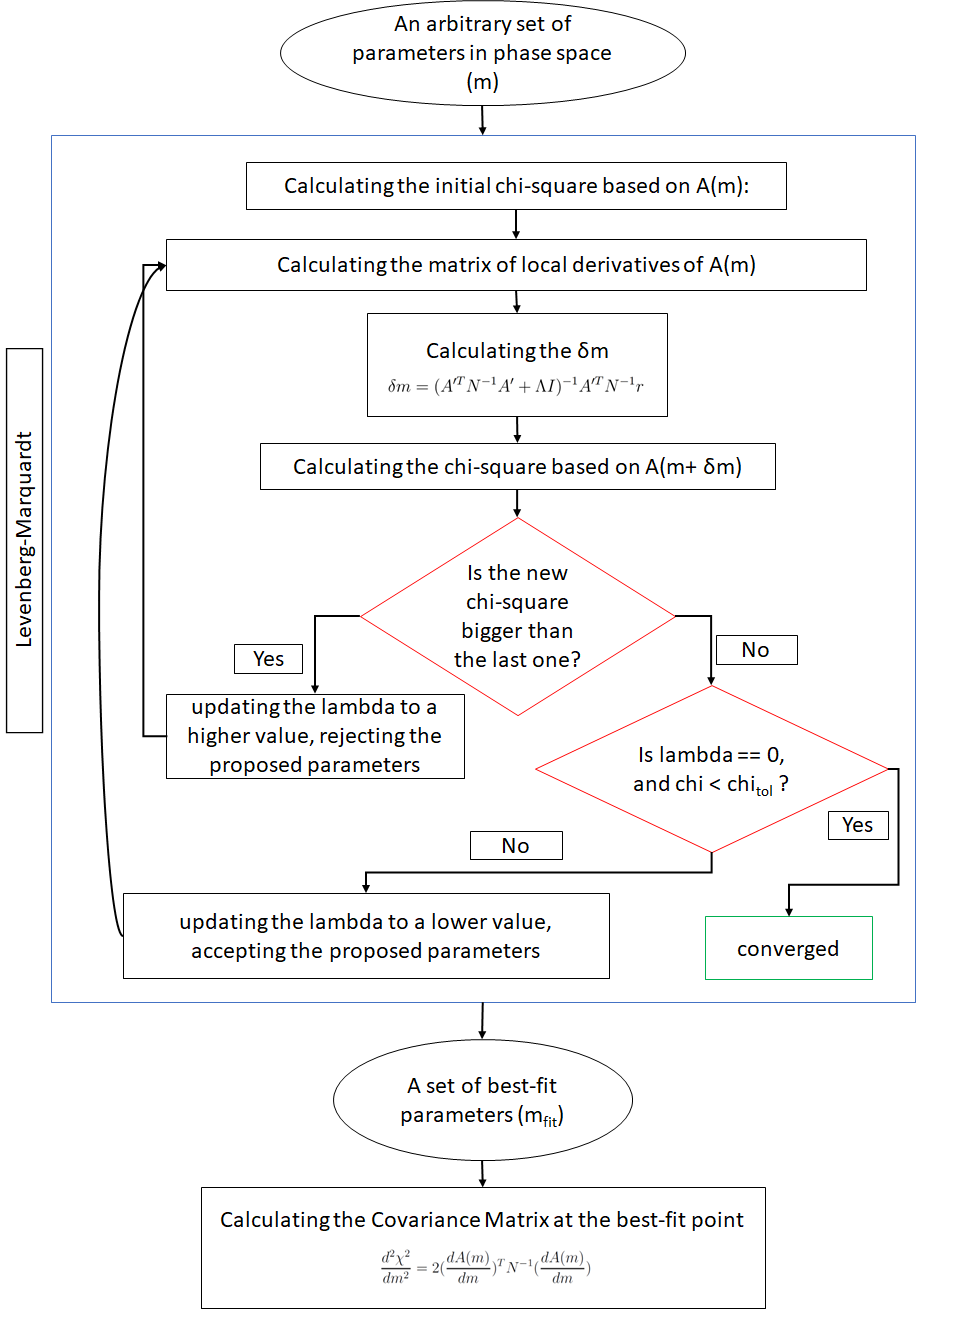
\includegraphics[scale =0.7]{LM_flow.png}
\caption[Flow chart of \gls{lm}]{Flow chart depicting the Levenberg-Marquardt algorithm. The algorithm starts with the calculation of the $\chi^2$ based on the theoretical model predicted by the initial set of parameters. Then, the new $\delta m$ is found using \ref{eq:LM}, and its associated $\chi^2$ is calculated. The new $\chi^2$ is compared to its value from the last iteration, and the value of the $\Lambda$ is determined by the success or failure of the current iteration. The algorithm is considered as converged if $\Lambda = 0$, and the $\chi^2$ decreases less than a threshold amount.}
\label{fig:LM_flow}
\end{figure}
%--------------------------------------------------------------------------------
\section{Markov Chain Monte Carlo (MCMC)}
Given that \gls{lm} is not always effective in finding the best-fit point for complex likelihood spaces, a more powerful algorithm such as \gls{mcmc} is necessary in many real-life applications. \gls{mcmc} is particularly effective in fitting non-Gaussian likelihood spaces and has a guaranteed convergence, regardless of the starting point in parameter space. However, the algorithm is computationally heavy due to its iterative nature, which is based on the evaluation of the chi-square on each step. Initially, an arbitrary point in parameter space is given to \gls{mcmc} as its initial trial step, and the associated chi-square is calculated. Then, a random point is drawn from a Gaussian distribution, where the mean is set at the last point in the chain\footnote{In Python applications, the numpy.randn function is used to serve this purpose.}. Subsequently, the new chi-square is compared to the previous one from the last trial step. If the new chi-square is lower, the new trial point is accepted into the chain. If the new chi-square is higher, the trial point is accepted with a probability determined by a specific criterion. This criterion is defined based on Gaussian insights:
\begin{equation}
    Probability = e^{\frac{-1}{2}\left(\chi_{new}^2 - \chi^2\right)} 
    \label{eq:mcmc_probability}
\end{equation}
As a measure of \gls{mcmc} convergence speed, the "acceptance ratio" is used to determine the fraction of trial steps that end up getting accepted into the chain. An ideal \gls{mcmc} would have an acceptance ratio of 25 percent. It should be noted that the convergence of the \gls{mcmc} is not dependent on the value of the acceptance ratio, but it influences the number of trial steps before the algorithm reaches its convergence. A low acceptance ratio will result in the need for more trial steps, therefore, a longer period of run-time.\par
A visual summary of \gls{mcmc} algorithm is illustrated in Figure \ref{fig:MCMC_flow}.
\begin{figure}[h!]
\centering
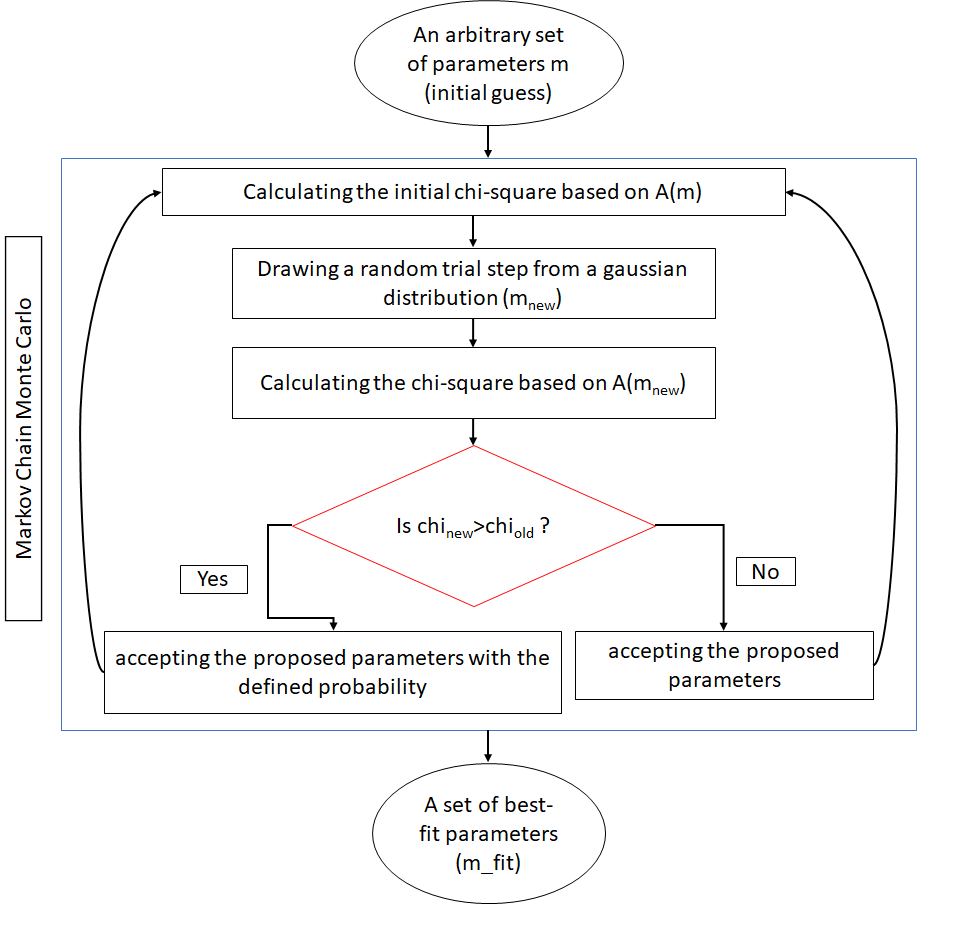
\includegraphics[scale =0.9]{MCMC_flow.png}
\caption[Flow chart of \gls{mcmc}]{Flow chart depicting the \gls{mcmc} algorithm. The algorithm starts with the calculation of the $\chi^2$ based on the theoretical model predicted by the initial set of parameters. Then, a new set of parameters are drawn from independent one-dimensional Gaussian distributions, and the associated $\chi^2$ is calculated. The new $\chi^2$ is compared to its value from the last iteration. If $\chi^2$ has lowered, the new combination of parameters is accepted into the chain. Otherwise, the parameters will be accepted by the probability defined in \ref{eq:mcmc_probability}. The algorithm itself does not contain control mechanisms to test its own convergence. Therefore, other approaches, such as power spectrum investigation, are employed (refer to section \ref{chap:method,sub:mcmc,subsub:convergence} and Figures \ref{fig:MCMC_converged} and \ref{fig:MCMC_unconverged}).}
\label{fig:MCMC_flow}
\end{figure}
%-----------------------------------------------------------------------------
\subsection{Convergence Test}
\label{chap:method,sub:mcmc,subsub:convergence}
The \gls{mcmc} algorithm requires to explore different regions of the parameter space in order to reach convergence. Various methods have been developed to ensure the convergence of this approach, one of which involves the investigation of the behavior of the power spectrum. The power spectrum represents the distribution of power at different frequencies in the \gls{mcmc} chain. In the case of a fully-converged \gls{mcmc} chain, the power spectrum must demonstrate the behavior of white noise, with power uniformly distributed among all frequencies. On the other hand, the power spectrum of an unconverged chain shows ascending power for lower frequencies. Therefore, the criterion for ensuring the convergence of an \gls{mcmc} is the flatness of the chain power spectrum in low frequencies when plotted on a log-log scale. Figure \ref{fig:MCMC_unconverged} and \ref{fig:MCMC_converged} illustrate the difference between a converged and an unconverged chain.\par
\begin{figure}[h!]
\centering
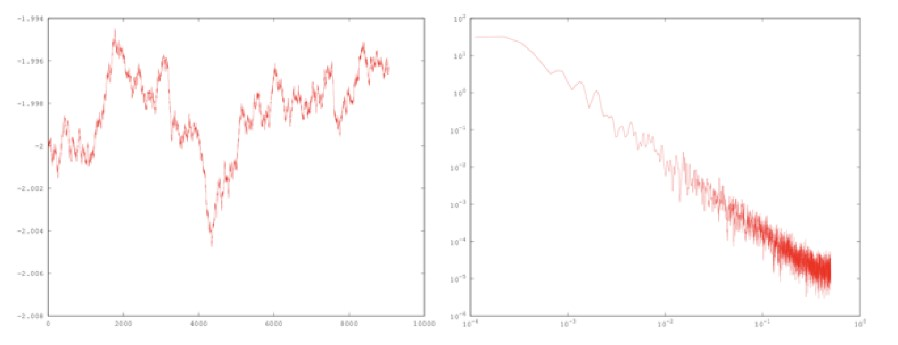
\includegraphics[scale =0.9]{mcmc_uncoverged.jpg}
\caption[An unconverged \gls{mcmc} chain and its power spectrum]{An unconverged \gls{mcmc} chain (left panel) and its power spectrum (right panel): A converged \gls{mcmc} chain is expected to exhibit the behavior of white noise. Thus, on the power spectrum, the power shall be uniformly distributed among different frequencies (after the burn-in phase of the \gls{mcmc}). Here, the power tends to increase in lower frequencies, and the chain itself does not indicate the behavior of white noise. Therefore, this chain is not yet converged. Figure from Jonathan Sievers \cite{mcmc_convergence_plot}}
\label{fig:MCMC_unconverged}
\end{figure}

\begin{figure}[h!]
\centering
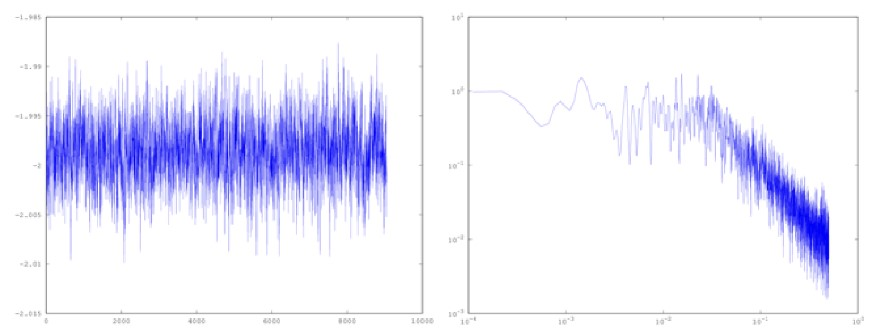
\includegraphics[scale =0.9]{mcmc_converged.jpg}
\caption[A converged \gls{mcmc} chain and its power spectrum]{A converged \gls{mcmc} chain (left panel) and its power spectrum (right panel): A converged \gls{mcmc} chain is expected to exhibit the behavior of white noise. Thus, on the power spectrum, the power shall be uniformly distributed among different frequencies (after the burn-in phase of the \gls{mcmc}). Here, the flat behavior of the power spectrum is evident, and the chain itself represents white noise. Figure from Jonathan Sievers \cite{mcmc_convergence_plot}}
\label{fig:MCMC_converged}
\end{figure}

%------------------------------------------------------------------------------------------------------
\section{Combination of MCMC and LM}
\gls{mcmc} is a computationally heavy algorithm due to its iterative nature. If the chi-square calculation process on each step is also a time-consuming task, the \gls{mcmc} will experience a rather long run-time before reaching the converged state. One of the proposed methods to deal with this issue and help the \gls{mcmc} to converge faster is to use the insights provided by the outputs of \gls{lm}. It is worth mentioning again that our sole rationale to use \gls{lm} in our application is to generate a covariance matrix for the \gls{mcmc}.\par
We previously discussed that the parameters of a model might be correlated with each other, and the strength of this correlation is dictated by the elements of the covariance matrix. During a basic \gls{mcmc} fitting process, we draw random samples from independent one-dimensional Gaussian distributions constructed for each of the parameters. These samples do not take the possible correlations of parameters into account. On the other hand, a modified \gls{mcmc}, which is combined with \gls{lm}, generates samples using a multivariate Gaussian distribution (joint normal distribution) and has the capacity to encompass such characteristics. This method will pave the way to increasing the probability of these samples getting accepted into the final chain. Eventually, we are able to summarize that this approach (feeding the \gls{mcmc} with a posterior distribution) will assist the \gls{mcmc} to explore more efficient regions of parameter space and converge faster. Figure \ref{fig:combined_flow} portrays this technique briefly.\par
The correlation between distinctive pairs of parameters can be visually assessed using \emph{corner plots}. A corner plot displays the pairwise scatter plots of all the parameters in the chain and it is particularly useful when dealing with high-dimensional parameter spaces. These plots provide insights to identify possible mutual dependencies. If there is a strong correlation between two parameters, it may indicate a degeneracy or a trade-off between those parameters in the model. Figure \ref{fig:corner_plots}, which shows the corner plots for a four-variable Gaussian model, emphasizes the importance of sampling from a multivariate normal distribution and taking the correlations between the parameters into account.\par
By utilizing the covariance matrix provided by the \gls{lm} algorithm, we possess the ability to generate an arbitrary number of correlated noise samples easily. The covariance matrix must be calculated at the point of "best fit" found by the \gls{lm}. This procedure is described thoroughly in the following section.\par

\begin{figure}[h!]
\centering
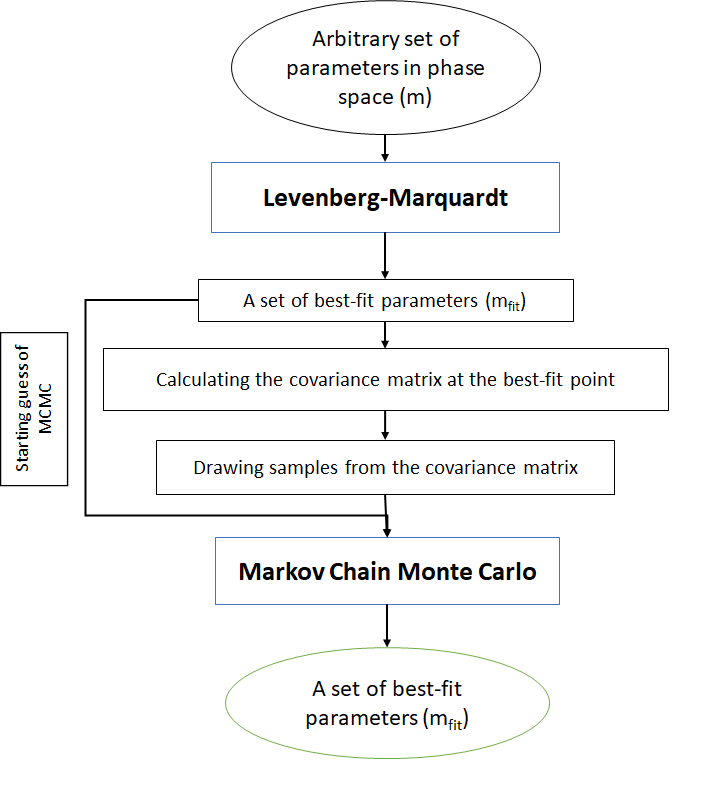
\includegraphics[scale =0.9]{combined_flow.png}
\caption[Flow chart of the procedure to combine \gls{mcmc} and \gls{lm}]{Flow chart of the procedure to combine \gls{mcmc} and \gls{lm}. We start with an arbitrary combination of parameters in phase space and run the \gls{lm} algorithm to find the best-fit point and the covariance matrix. Then, we draw sufficient samples from the covariance matrix to use them as the posterior distribution of our \gls{mcmc}. Eventually, the output of this combined method is a set of best-fit parameters and their associated error bars.}
\label{fig:combined_flow}
\end{figure}

\subsection{Generating Correlated Noise}
\label{chap:method,sub:correlated noise}
Correlated noise, as opposed to white noise, refers to a type of noise or random variation in a set of samples that exhibits a correlation or relationship with another variable. In other words, it is a noise that is not completely random but instead has some level of dependency on other parameters. The mathematical tool to quantify these correlations is the covariance matrix, which is often used to characterize the statistical properties of the noise. \par
The off-diagonal elements of a covariance matrix correspond to the covariance between each pair of parameters. Thus, by drawing samples from the covariance matrix, we are genuinely sampling from the multivariate normal distribution with the deviation values describing the uncertainties in the parameters.
Two equivalent approaches can be used to generate correlated noise: Cholesky and eigenvalue decomposition of the covariance matrix. For practical reasons, we prefer to use the eigenvalue decomposition for our applications\footnote{Normally, calculating the Cholesky decomposition takes a shorter amount of time.}. The procedure is as follows: A matrix of random variables drawn from a one-dimensional Gaussian is constructed in the desired shape ($n \times m$, corresponding to the number of samples and the number of parameters, respectively). Then, this matrix is multiplied by the eigenvalue matrix and scaled by the square root of the eigenvalues. The transposition of the product will provide the desired correlated samples. \par
To gain more precision, it is possible to use the eigenvalues decomposition of the normalized covariance matrix (where diagonal samples all equal unity). The normalization process is done by multiplying the covariance matrix with its own diagonal. Eventually, the drawn samples are denormalized by scaling them with the square root of the diagonal matrix.\par
\begin{figure}[h!]
\centering
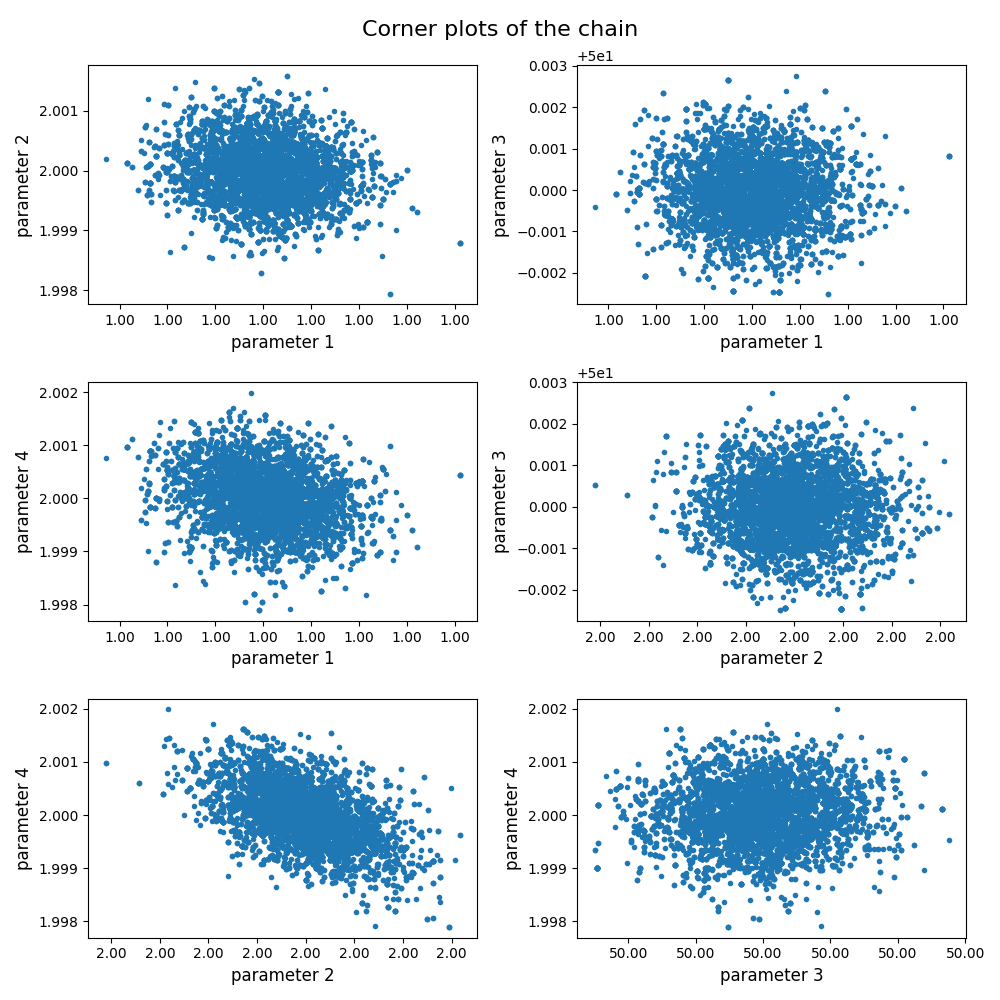
\includegraphics[scale =0.6]{corner_plots.png}
\caption[Corner plots of an \gls{mcmc} chain]{Corner plots (pairwise parameter contours) of a typical \gls{mcmc} chain from a four-variable Gaussian model. 
 A corner plot is the pairwise scatter plots of all the parameters in a \gls{mcmc} chain, providing a visual assessment of the correlation between parameters. These plots are especially advantageous in dealing with high-dimensional parameter spaces. Corner plots are also capable of identifying possible degeneracies. In this figure, the lower right panel clearly shows patterns of correlation between a pair of parameters. Sampling from a multivariate normal distribution based on the covariance matrix associated with these samples will take the correlations into account.}
\label{fig:corner_plots}
\end{figure}

\section{Algorithm Validation}
\label{chap:method,sub:test}
To ensure the accuracy and reliability of the results produced with the described algorithm, we present two distinctive validation tests. The criterion will also assess the performance of the algorithm and the overall quality of the model fitting.\par

\subsection{The Chi-Square Consistency Test}
\label{chap:method,sub:test,subsub:chi}
The primary focus of this approach lies in examining the results obtained from the \gls{lm} and the associated drawn samples. Numerous samples are drawn from the covariance matrix, and their corresponding chi-square is computed. Given that the covariance matrix holds the information on parameter uncertainties, it is anticipated that, on average, the disparity in chi-square statistics between two distinct samples should be roughly equivalent to one unit per each parameter of the model. This expectation arises from the fact that the chi-square statistic scales according to the uncertainties inherent in both the data and model, which have magnitudes around one.\par
Figure \ref{fig:csq_test} shows an example of the distribution of disparity between the chi-square values.\par
\begin{figure}[h!]
\centering
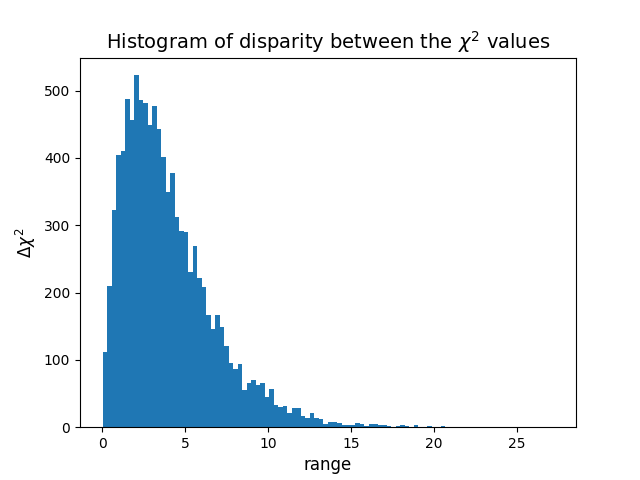
\includegraphics[scale =0.8]{csq_hist.png}
\caption[Histogram of disparity in the chi-square values of drawn samples]{Histogram illustrating the distribution of the disparity between the chi-squares of drawn samples for a four-variable Gaussian model. The samples are drawn from the covariance matrix calculated at the point of best fit (output of \gls{lm}). We expect the average difference in the $\chi^2$ statistics for two different samples to be of order unity per each parameter.
On this plot, the average of disparity is 4.03, and the standard deviation is 2.83, in acceptable agreement with our expectations. Therefore, the best-fit parameters are considered a "good fit".}
\label{fig:csq_test}
\end{figure}
\subsection{The Chi-Square Parameter Correlation Test}
\label{chap:method,sub:test,subsub:plot}
An alternative approach for result verification involves creating plots that depict the relationship between the chi-square values of drawn samples and individual parameters. With reference to the defined chi-square equation (see Equation \ref{eq:chi-square matrix}), which captures the non-linear dependence of chi-square on model parameters, it is anticipated that a parabolic trend will be observed. Figure \ref{fig:csq_params} illustrates plots of chi-square values against parameters for the identical mathematical model as presented in Figure \ref{fig:csq_test}. \par
\begin{figure}[h!]
\centering
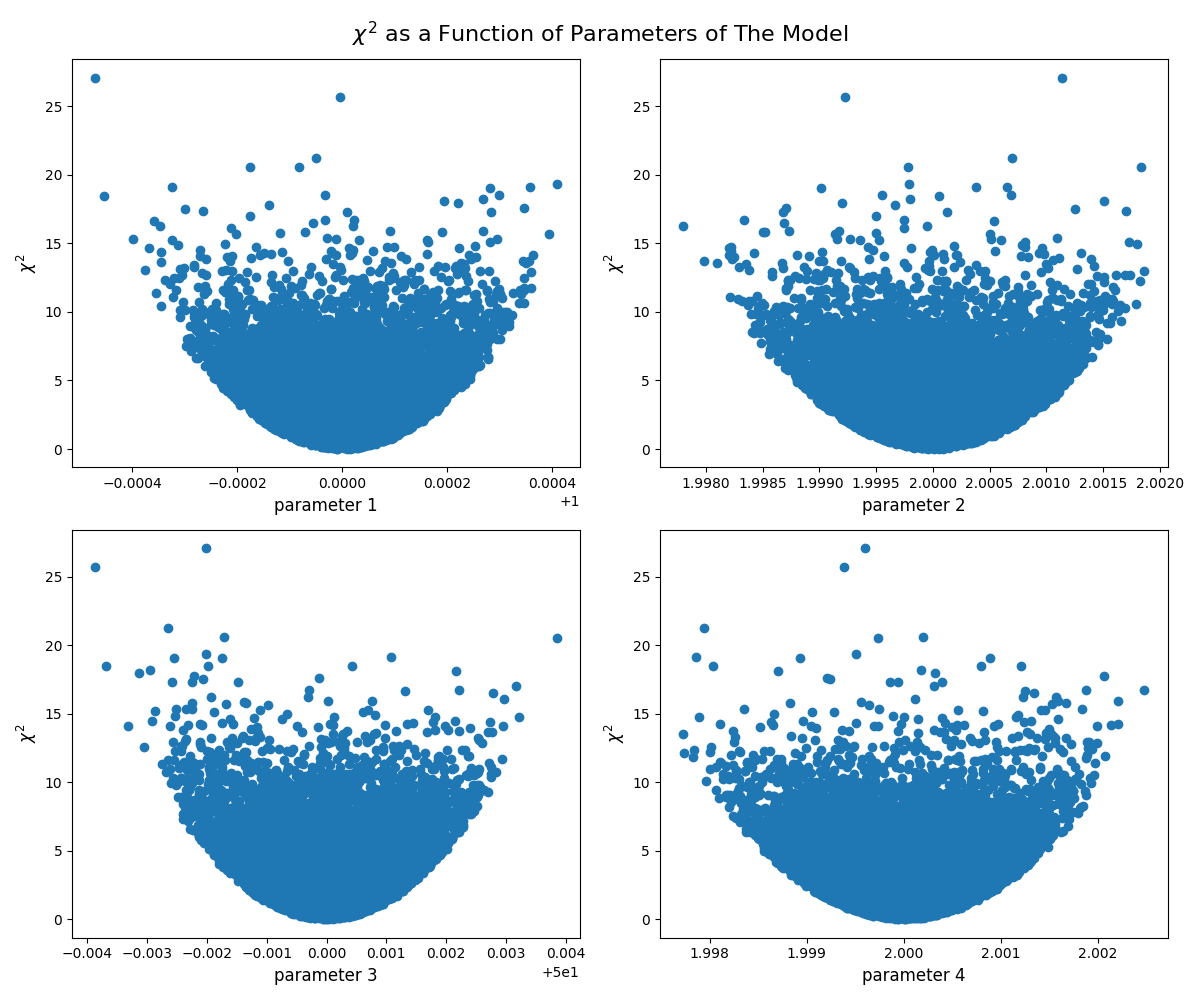
\includegraphics[scale =0.5]{csq_vs_params.png}
\caption[Chi-Square vs. parameters plots]{Figures demonstrating the values of chi-square associated with the drawn samples versus the values of parameters for a four-variable Gaussian model. The $\chi^2$ is expected to have a parabolic dependency on the value of parameters based on its non-linear definition (\ref{eq:chi-square matrix}). This is a test to confirm the accuracy of the covariance matrix and the procedure of sample drawing.}
\label{fig:csq_params}
\end{figure}
%###################################################################################
\chapter{Results and Analysis}
\label{chap:results}
Following the discussions of chapter \ref{chap:method} to formulate a specific data fitting algorithm based on the synchronized utilization of \gls{lm} and \gls{mcmc}, this chapter is devoted to demonstrating the results of applying this method to the global $21cm$ signal. As an example, we offer a theoretical best-fit curve for the \gls{edges} data. \par
An essential step in the process of model fitting is to determine the parameters of the physical model. As we choose to use \gls{ares} for generating the theoretical curve, the parameterization of theory is restricted to the notation employed by \gls{ares}. We will briefly introduce our chosen parameters and revisit their connection to the underlying physics of the $21cm$ line. We proceed by evaluating the quality of fit by estimating the parameters of a mock data set, which in fact, is an \gls{ares}-generated curve. The reliability of the results is proven by considering the values of estimated parameters and the assumed error bars of the mock data. \par
Finally, we represent the results of parameter estimation for \gls{edges} data. \hl{These results will show us that the anomalous behavior of this data (with respect to theoretical expectations) is an obstacle to providing a fit to this signal.}\par
\section{Key Astrophysical Parameters}
Based on the discussions of \ref{chap:global21cm,sub:physics}, the shape and amplitude of global $21cm$ signal are intensely dependent on underlying astrophysical processes, especially those related to the \gls{sfr} and reheating of the \gls{igm}. In this section, we will take the discussion further and address our current understanding of this dependency on four specific parameters which are able to map the parameter space of the global $21cm$ signal effectively. Constraining these parameters will result in improved comprehension of the thermal history of the \gls{igm} and the population of X-ray sources during high-redshift epochs \cite{21century}.\par
It is essential to mention that although it is theoretically possible to investigate the cosmological parameters with this signal as well (refer to equation \ref{eq:global_curve} for the exact dependency of the global curve on cosmological parameters), the accuracy of the observational data is yet insufficient for constraining these parameters. Moreover, the $21cm$ signal is the only identified prob for some specific astrophysical mechanisms during the dark ages and \gls{eor}, while cosmological parameters can be studied using \gls{cmb} as well. Therefore, we introduce four astrophysical parameters hereunder, which will form the basis of our analysis. \par
\begin{enumerate}
    \item \bm{$f_X$}: \emph{High-redshift proportionality constant in X-ray luminosity and \gls{sfr} relation} \cite{ares_documentation}. 
    X-ray photons generated by galaxies and quasars are likely the most important cause of heating the low-density IGM \cite{low_frequency}. Considering the fact that the nature of high-redshift objects is not properly studied, it is not possible to give an exact theory for the high-redshift X-ray background. The safest course of action is to assume that the relation between X-ray luminosity and \gls{sfr} in high redshift contains a proportionality constant $f_X$ which ascends with redshift\footnote{The primordial mass function is strongly weighted toward the high-redshift end, so the proportionality constant between X-ray production and \gls{sfr} is larger at high-redshift.}.
    \begin{equation}
        L_X = 3.4 \times 10^{40} f_X \left( \frac{SFR}{1 \hspace{0.1cm} M_{\odot} \hspace{0.1cm} yr^{-1}}\right) \hspace{0.1cm} erg \hspace{0.1cm}s^{-1}
    \end{equation}
    The normalization was chosen such that, when $f_X =1$, the total X-ray luminosity per unit \gls{sfr} is consistent with that observed in starburst galaxies at the present epoch \cite{low_frequency, 21century}.
    
    \item \bm{$N_{lw}$}: \emph{Number of photons emitted in the Lyman-Werner band ($11.5eV<E<13.6eV$) per baryon of star formation}. This parameter is referred to as \emph{pop\_rad\_yield\_0\_} in ARES documentation \cite{ares_documentation, lw_background}
    
    \item \bm{$N_{ion}$}: \emph{Mean number of ionizing photons ($E>13.6eV$) produced per baryon of star formation}. This parameter is referred to as \emph{pop\_rad\_yield\_2\_} in ARES documentation \cite{ares_documentation, 21century}
    
    \item \bm{$f_{esc}$}: \emph{Fraction of ionizing photons that escape their host galaxy into the \gls{igm}} \cite{ares_documentation}.
    $f_{esc}$ and $N_{ion}$ are both defined in the process of calculating the evolution of ionization fraction $\bar{x}_i$:
    \begin{gather}
        \bar{x}_i = \frac{\zeta f_{coll}}{1 + \bar{n}_{rec}}\\
        f_{coll} = \int_{m_{min}}^\infty dm \hspace{0.1cm} m \hspace{0.1cm} n\left(m\right)\\
        \xi_{\text{ion}} = A_{He} \hspace{0.1cm} f_* \hspace{0.1cm} f_{esc} \hspace{0.1cm} N_{\text{ion}} \label{eq:ionizing_efficiency}
    \end{gather}
    
    $f_{coll}$ is the collapse fraction (fraction of gas inside collapsed objects, fraction of mass in halos more massive than $m_{min})$, $\bar{n}_{rec}$ is the mean number of recombinations per ionized hydrogen atom, $\xi_{\text{ion}}$ is the ionizing efficiency, $f_*$ is the star formation efficiency (fraction of baryons converted into stars), and $A_{He} = 4/(4 - 3Y_p) = 1.22$. The mass fraction of helium, $Y_p$, is a correction factor to convert the number of ionizing photons per baryon in stars to the fraction of ionized hydrogen. Our limited understanding of the mass distribution of the emitting stars introduces an uncertainty in the number of ionizing photons per baryon $N_{ion}$, that is emitted by galaxies. There is also considerable uncertainty in the fraction of ionizing photons $f_{esc}$ that escape the host galaxy to ionize the \gls{igm}. Therefore, our study is toward the urgent demand to constrain these parameters with observational data \cite{low_frequency, 21century}.\par
    Alternatively, we could have utilized $f_*$ as a parameter of our model. However, since $f_{esc}$ and $N_{ion}$ act as multiplication factors to $f_*$ in the expression for ionizing efficiency \ref{eq:ionizing_efficiency}, thus, both of them are individually degenerate with star formation rate.
\end{enumerate}
Figure \ref{fig:sensivity} shows the influence of change in the values of the above-mentioned parameters on the global $21cm$ curve generated by \gls{ares}. It must be noted that these parameters are only physically meaningful in a limited region of phase space (A hypercube where the combination of parameters is physically meaningful). Going beyond this region will result in a failure in calculating the global $21cm$ curve. our developed script is designed to handle this issue and stop it from aborting the whole run \footnote{The Python code for the \gls{mcmc} is designed such that it will return an arbitrarily large chi-square for that combination of parameters beyond the permitted hypercube. Therefore, the probability of these points getting accepted into the chain will be automatically low.}, but the \gls{mcmc} might not be able to reach convergence if the algorithm faces numerous samples beyond the allowed region.\par
%-----------------------------------------------------------------------------------
\section{Parameter Estimation of Mock Data}
\label{chap:results,sub:known_curve}
Prior to applying our developed algorithm to fit real-world data, we perform a validation test by using it to fit a mock data set. We create an \gls{ares} curve based on a predetermined set of parameters, treating it as mock data with an assumed error bar of $10^{-3}K$ on each data point. We confirm the correct functioning of the algorithm by comparing the obtained fitted parameters to the expected values.\par
The results of this validation test are shown in Table \ref{tab:mcmc_results_known_curve}. The initial row contains the genuine parameters employed in generating the mock data, while the second row exhibits the fitting outcome. Subsequently, the third row displays the one-sigma error bar of the fit, which is based on the standard deviation of \gls{mcmc} chain. The last row demonstrates the relative fitting error, which serves as a measure for assessing the disparity between the true values of astrophysical parameters and their corresponding fit.\par 
Figure \ref{fig:fit_curve_known_curve} is the illustration of the data in table \ref{tab:mcmc_results_known_curve}. 
The blue dotted curve and the red curve on the left panel depict the mock data and the corresponding fit, respectively.
On the other hand, the right panel, which is the zoomed version of the same plot, demonstrates the two-sigma confidence interval of the fit. The overall output is an acceptable fit considering both the shape and amplitude of the signal.\par
Figure \ref{fig:chain_known_curve} indicates the white-noise behavior of parameters throughout the chain, which is in agreement with our anticipation for a converged chain. Performing \emph{chi-Square consistency test} on our samples showed that the average disparity between the chi-square of drawn samples is 49.20, roughly an order of magnitude larger than the initial expectation ($\approx4$) (refer to Figure \ref{fig:csq_test}). The \emph{chi-square parameter correlation test} (Figures \ref{fig:csq_vs_params_knwon_curve}) did not show parabolic behavior initially. However, Figure \ref{fig:csq_vs_params_zoomed_known_curve}, which demonstrates the zoomed version of the \ref{fig:csq_vs_params_knwon_curve}, gives insights on parabolic behavior for lower values of chi-square. Figure \ref{fig:corner_plots_known_curve} illustrates the corner plots of this chain. The lower left panel indicates that the $f_X$ and $pop\_rad\_ yield\_2$ have the highest amount of correlation in all pairs of parameters.\par

\begin{table}
\centering
\caption[Results of fitting a mock data set]{Results of fitting a mock data set with \gls{mcmc} chain. The first row is the actual parameters used to generate the mock data. The second row is the fit value of the same astrophysical parameters. The third row is the one-sigma error bar of fit, and eventually, the fourth row represents the relative fitting error which is a measure of disparity between the values of the first and second rows.}
\label{tab:mcmc_results_known_curve}
\begin{tabular}{|c|c|c|c|c|}
\hline
\diagbox{Value}{Parameter} & \emph{pop\_rad\_yield\_0\_} & \emph{pop\_rad\_yield\_2\_} & \emph{$f_{esc}$} & \emph{$f_X$}\\
\hline
True values & $1 \times 10^ {4}$ & $1 \times 10^ {3}$ & 0.1 & 0.1\\
\hline
Fitted values & $9.9999 \times 10^ {3}$ & $9.9941 \times 10^ {2}$ & $1.0002 \times 10^ {-1}$ & $1.0000 \times 10^ {-1}$ \\
\hline
Error-bar of fit & $3.4727 \times 10^ {-2}$ & $3.8932
\times 10^ {0}$& $3.6299 \times 10^ {-4}$ & $3.3186 \times 10^ {-6}$ \\
\hline
Fitting Error & 0.0001\% & 0.0264 \%& 0.0152\%& 0.0003\%\\
\hline
\end{tabular}
\end{table}
%-----------------------------------------------------------------------------------
\section{Parameter Estimation of EDGES data}
This section demonstrates the results of applying our developed method to the \gls{edges} data, which is the only claimed observational data set of the global $21cm$ signal. 
We formerly discussed that standard physical mechanisms are unable to explain the large amplitude of this data as it is roughly more than two times higher than the most optimistic theoretical curves. On the other hand, \gls{ares}, which generates the theoretical global $21cm$ curve, is based on the predictions of standard physics. Therefore, in order to gain a more realistic fit of the \gls{edges} data, we tend to use a suppressing multiplication factor which draws the amplitude of the data to half of its original value. Furthermore, as a matter of convenience in the first-step analysis, we refrain from employing the actual noise model used by the \gls{edges} group. Instead, we approximate the noise using the radiometer equation. The details of this approach is presented in section \ref{chap:results,sub:edges,subsub:error}.\par

\subsection{Error Bar Calculation}
\label{chap:results,sub:edges,subsub:error}
In order to obtain the error bars of the \gls{edges} data for the parameter estimation process, it is possible to use the \gls{edges} noise model directly. Another option is to take advantage of the approximation provided by the radiometer equation, which expresses the sensitivity of a radio antenna \cite{sensitivity_1, sensitivity_2}.\par
\begin{equation}
    \frac{\delta T}{T_{sys}} = \frac{1}{\sqrt{Bt}}
\end{equation}
Where B is the bandwidth, t is the exposure time, and $T_{sys}$ is the system temperature. Assuming a bandwidth of $10^6Hz$, an exposure time of one day, and a temperature of $3000K$, we get
\begin{equation}
   \delta T_{EDGES} = 10 ^{-2}K = 10mK. 
\end{equation}

\subsection{Results}
The outcomes obtained by applying our methodology to the \gls{edges} data are presented in Table \ref{tab:mcmc_results_edges}. In the first row, the best-fit parameters for the half-amplitude data are displayed. Subsequently, the second row exhibits the one-sigma error bar of the fit, derived from the standard deviation of the \gls{mcmc} chain. \par
Figure \ref{fig:fit_curve_edges} is the visual demonstration of the data from Table \ref{tab:mcmc_results_edges}, with the blue dotted curve representing the data and the red curve portraying the corresponding fit on the left panel. The right panel, being a zoomed version of the same plot, illustrates the two-sigma confidence interval of the fit. The overall findings reveal a notable discrepancy when compared to the observed data, suggesting the implausibility of achieving the \gls{edges} curve by solely considering the expectations of standard physics.\par
Figure \ref{fig:chain_edges} shows the white-noise behavior of parameters throughout the chain, confirming that it has converged. The performed \emph{chi-square consistency test} on the samples indicated an average disparity of 0.28 between the chi-square values of the drawn samples, significantly lower (roughly two orders of magnitude) than the initial expectation of approximately 4. The \emph{chi-square parameter correlation test} (Figures \ref{fig:csq_vs_params_edges}) revealed parabolic behavior only for parameters $pop\_rad\_yield\_2$ and $f_X$. However, upon examining the zoomed version of Figure \ref{fig:csq_vs_params_edges} in Figure \ref{fig:csq_vs_params_zoomed_edges}, it became evident that the two remaining parameters also exhibit parabolic behavior at lower values of chi-square.\par
The chain's corner plots are depicted in Figure \ref{fig:corner_plots_edges}. Among all six panels, the middle left panel, which represents the values of $f_X$ and $pop\_rad\_yield\_0$, demonstrates the only noticeable correlation between a pair of parameters.
 
\begin{table}[h!]
\centering
\caption[Results of fitting \gls{edges} data with \gls{mcmc} chain]{Results of fitting \gls{edges} data with \gls{mcmc} chain. The upper row is the fit value of four astrophysical parameters of the model, and the lower row is the one-sigma error bar of fit.}
\label{tab:mcmc_results_edges}
\begin{tabular}{|c|c|c|c|c|}
\hline
\diagbox{Value}{Parameter} & \emph{pop\_rad\_yield\_0\_} & \emph{pop\_rad\_yield\_2\_} & \emph{$f_{esc}$} & \emph{$f_X$}\\
\hline
Fitted values & $4.5493 \times 10^ {3}$ & $2.4759 \times 10^ {3}$ & $3.7010 \times 10^ {-1}$ & $1.3639 \times 10^ {-1}$ \\
\hline
Error-bar of fit & $1.8083 \times 10^ {-1}$ & $7.6298 \times 10^ {1}$& $1.1408 \times 10^ {-2}$ & $6.5033\times 10^ {-6}$ \\
\hline
\end{tabular}
\end{table}

% -------------------------------------------------------------------------------------
\begin{figure}[h!]
\centering
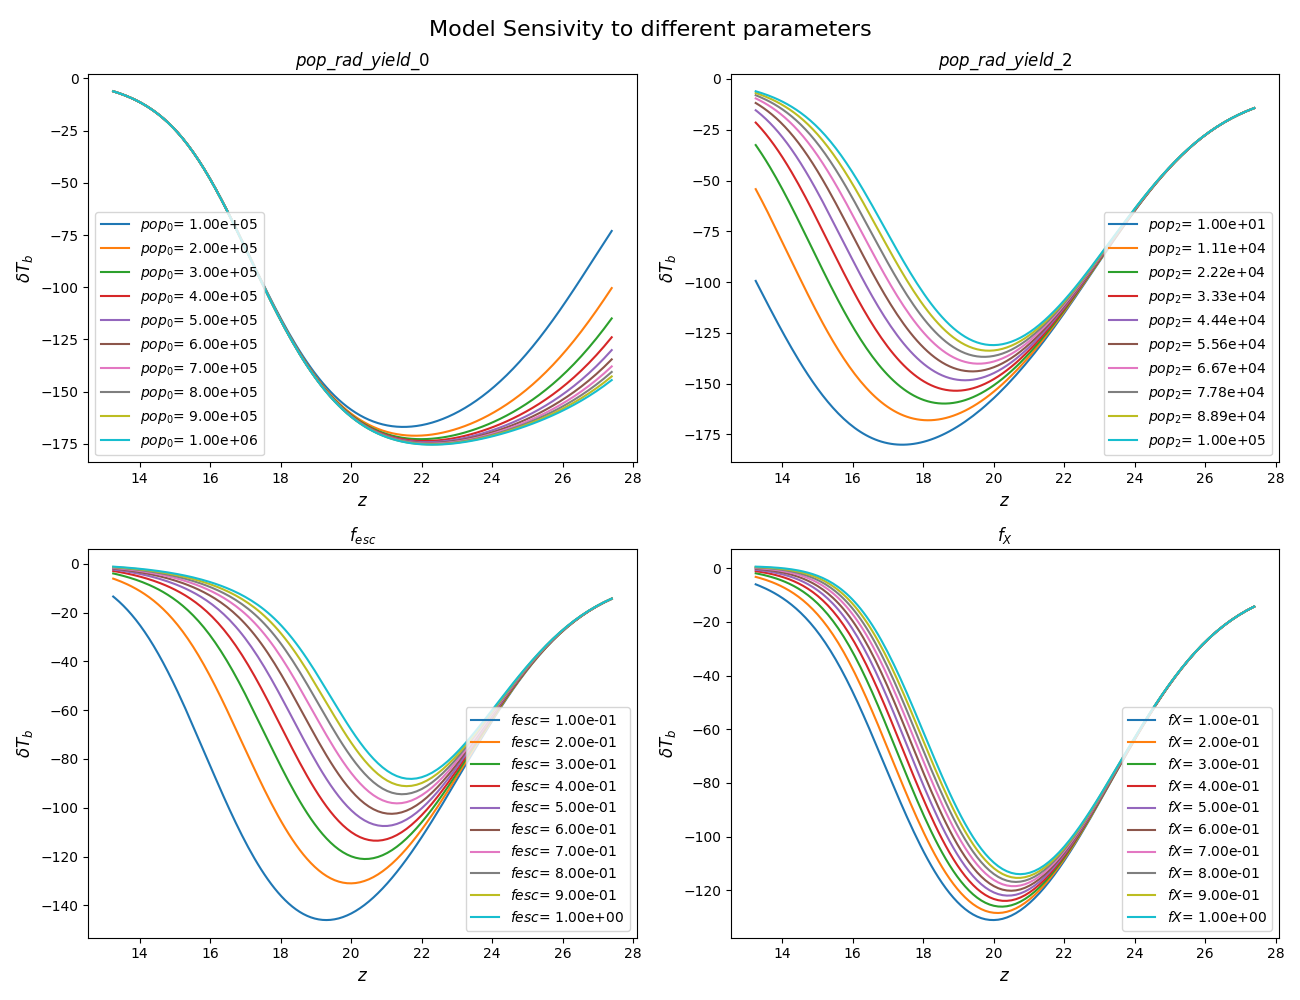
\includegraphics[scale =0.5]{sensivity.png}
\caption[Behaviour of global $21cm$ theoretical model with respect to underlying astrophysical parameters]{Behaviour of ARES-generated global $21cm$ models with respect to four astrophysical parameters: \emph{pop\_rad\_yield\_0\_}, \emph{pop\_rad\_yield\_2\_}, $f_{esc}$, and $f_X$. In each panel, the corresponding parameter possesses 10 different values, and other parameters are kept at the values of  $10^4$, $10^5$, $0.2$, and $0.1$, respectively. Each parameter is capable of affecting the shape and depth of the absorption trough.}
\label{fig:sensivity}
\end{figure}
%@@@@@@@@@@@@@@@@@@@@@@@@@@@@@@@@@@@@@@@@@@@@@@@@@@@@@@@@@@@@@@@@@@@@@@@@@@
\begin{figure}[h!]
\centering
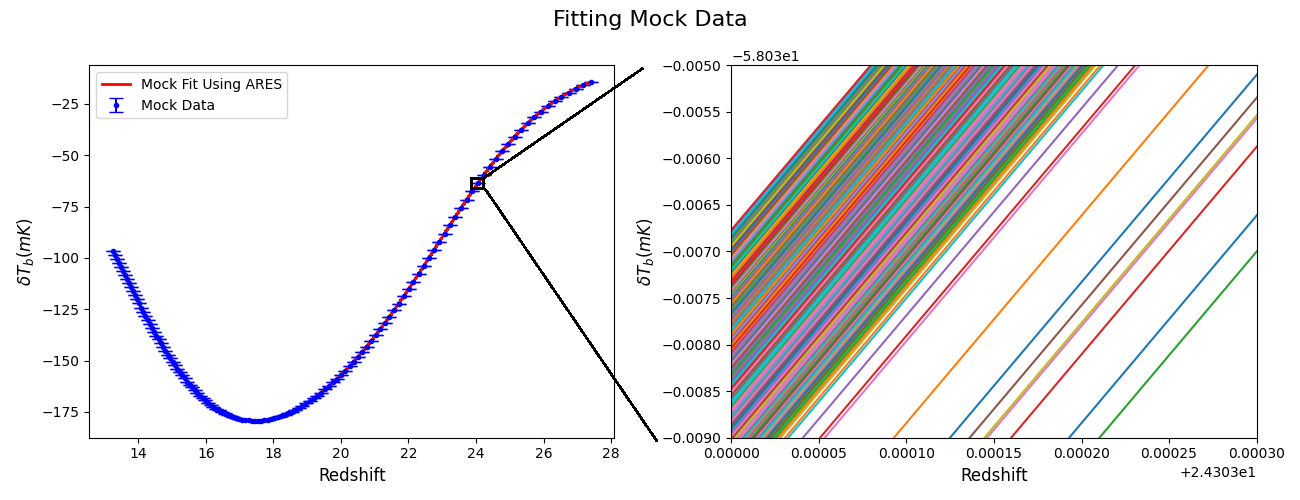
\includegraphics[scale =0.7]{fit_curve_mock.png}
\caption[Results of fitting mock data]{Results of fitting mock data. On the \textbf{left panel}, the blue dotted curve represents the mock data and the assumed uncertainty ($10^{-3}K$) generated by feeding the parameters of table \ref{tab:mcmc_results_known_curve} to \gls{ares}. The red curve demonstrates the fit curve, which is an excellent fit to the data, further validating the developed fitting method. The \textbf{right panel} is the zoomed version of the left figure, showing the two-sigma confidence interval of the fit (8698 curves), which is not visible on the left.}
\label{fig:fit_curve_known_curve}
\end{figure}

\begin{figure}[h!]
\centering
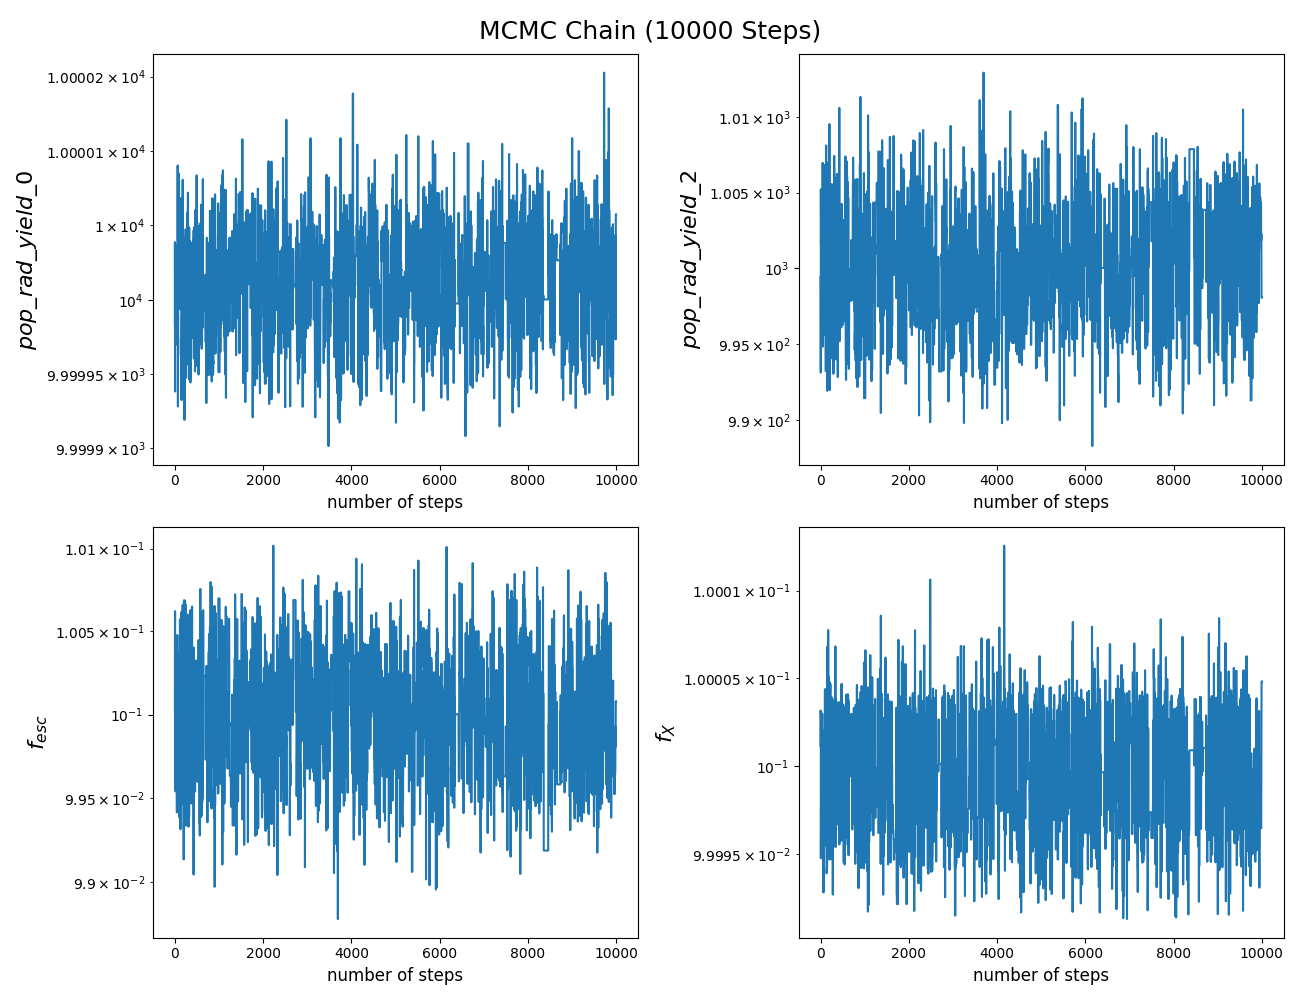
\includegraphics[scale =0.5]{chain_known_curve.png}
\caption[Trend of parameters in the mock data \gls{mcmc} chain]{Trend of parameters in the $10^4$ steps \gls{mcmc} chain to fit the mock data. The depicted white noise behavior is considered as the sign of the convergence of the \gls{mcmc} chain (refer to \ref{chap:method,sub:mcmc,subsub:convergence}). The acceptance ratio of the chain is $20.5\%$, close to the ideal of $25\%$. The one-sigma error bar of the fit (table \ref{tab:mcmc_results_known_curve}) is the standard deviation of this chain.}
\label{fig:chain_known_curve}
\end{figure}

\begin{figure}[h!]
\centering
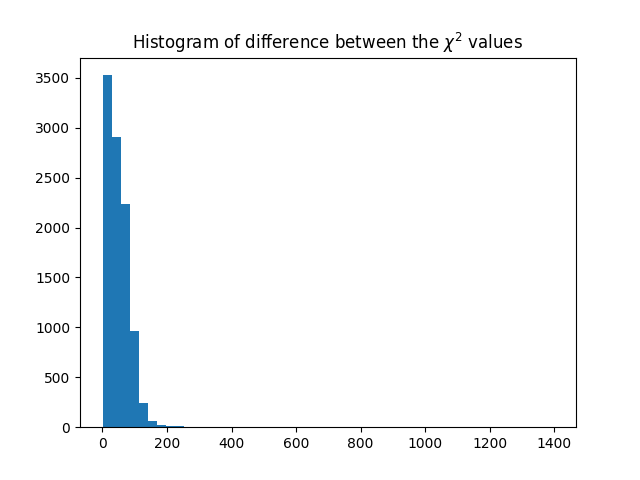
\includegraphics[scale =0.7]{csq_hist_known_curve.png}
\caption[Histogram of disparity in the chi-square of drawn samples for the mock data \gls{mcmc} chain]{Histogram of disparity in the Chi-Square of drawn samples for the mock data \gls{mcmc} chain, the mean is 49.20 with a standard deviation of 41.98. Based on the discussions of \ref{chap:method,sub:test,subsub:chi}, we expected the mean to be approximately 4.}
\label{fig:csq_hist_known_curve}
\end{figure}

\begin{figure}[h!]
\centering
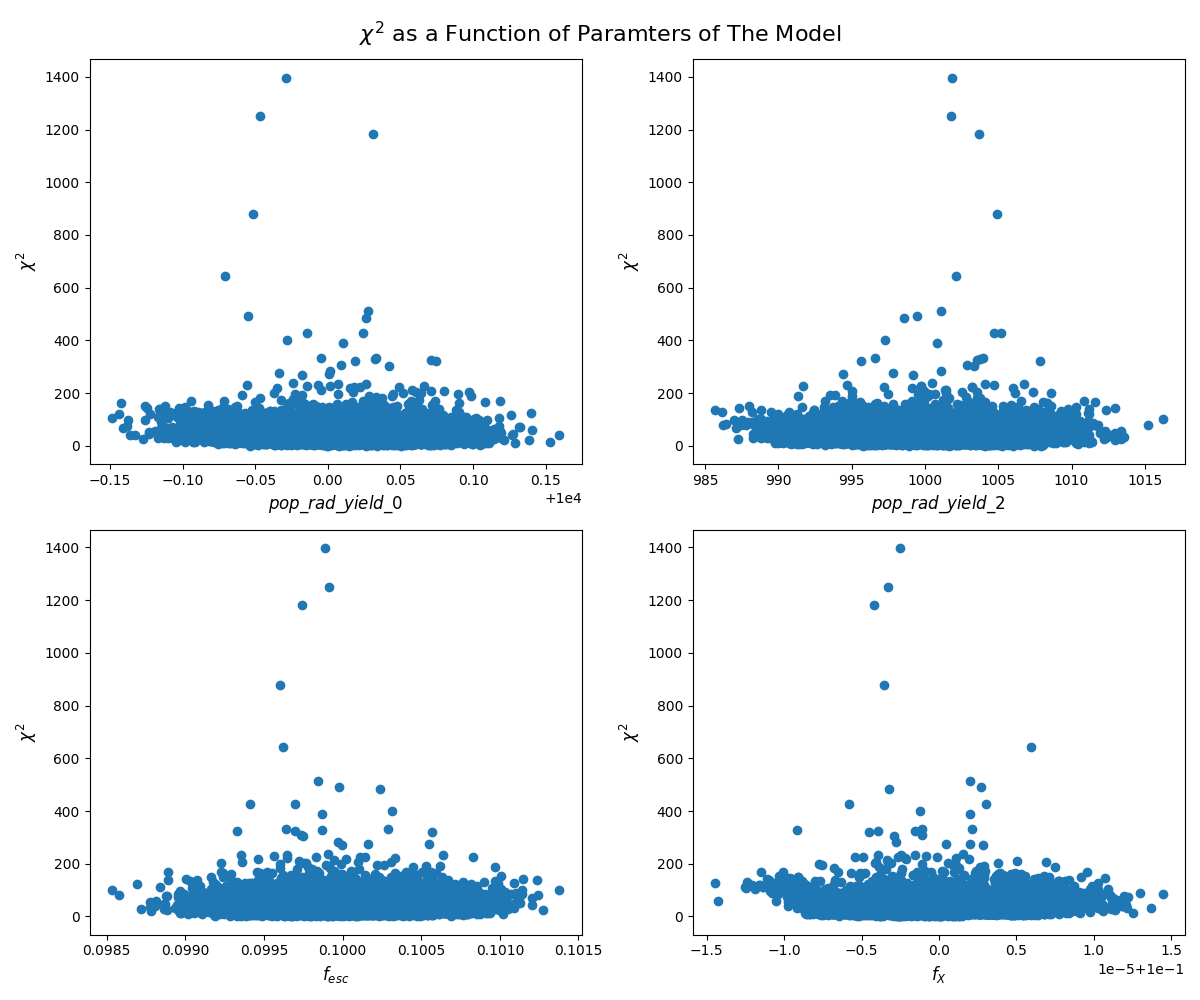
\includegraphics[scale =0.5]{csq_vs_params_known_curve.png}
\caption[Chi-Square of Drawn samples as a function of parameter values for the mock data]{Figures demonstrating the values of chi-square associated with the drawn samples versus the values of parameters for the mock data set. The $\chi^2$ is
expected to have a parabolic dependency on the value of parameters. However, the parabolic behavior is not obvious in these plots.}
\label{fig:csq_vs_params_knwon_curve}
\end{figure}

\begin{figure}[h!]
\centering
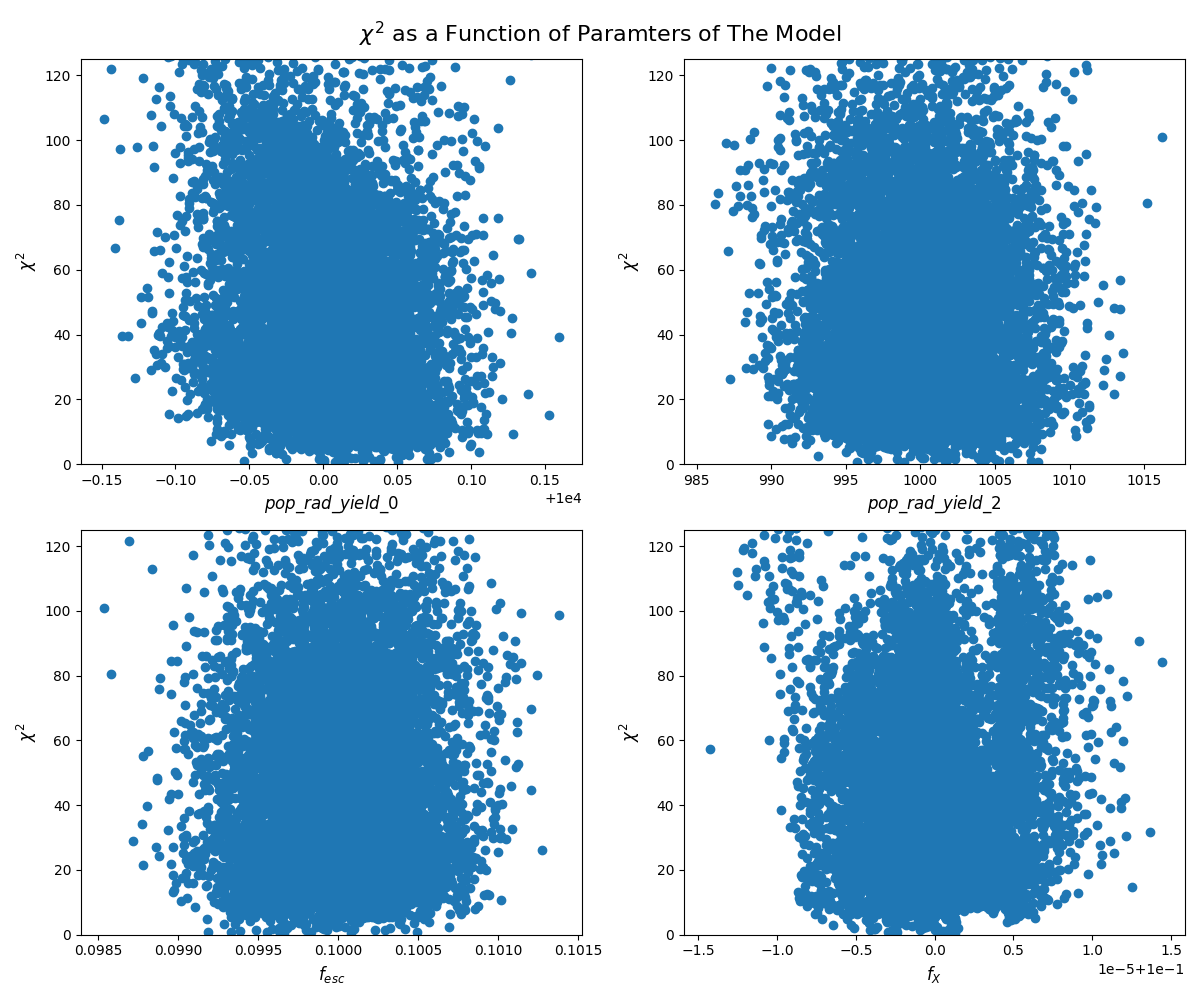
\includegraphics[scale =0.5]{csq_vs_params_zoomed_known_curve.png}
\caption[Chi-Square of Drawn samples as a function of parameter values for the mock data, zoomed version]{Zoomed version of figure \ref{fig:csq_vs_params_knwon_curve}, A weak parabolic behaviour is observed for low values of $\chi^2$. However, the overall shape is not completely consistent with the expectations of Figure \ref{fig:csq_params}.}
\label{fig:csq_vs_params_zoomed_known_curve}
\end{figure}


\begin{figure}[h!]
\centering
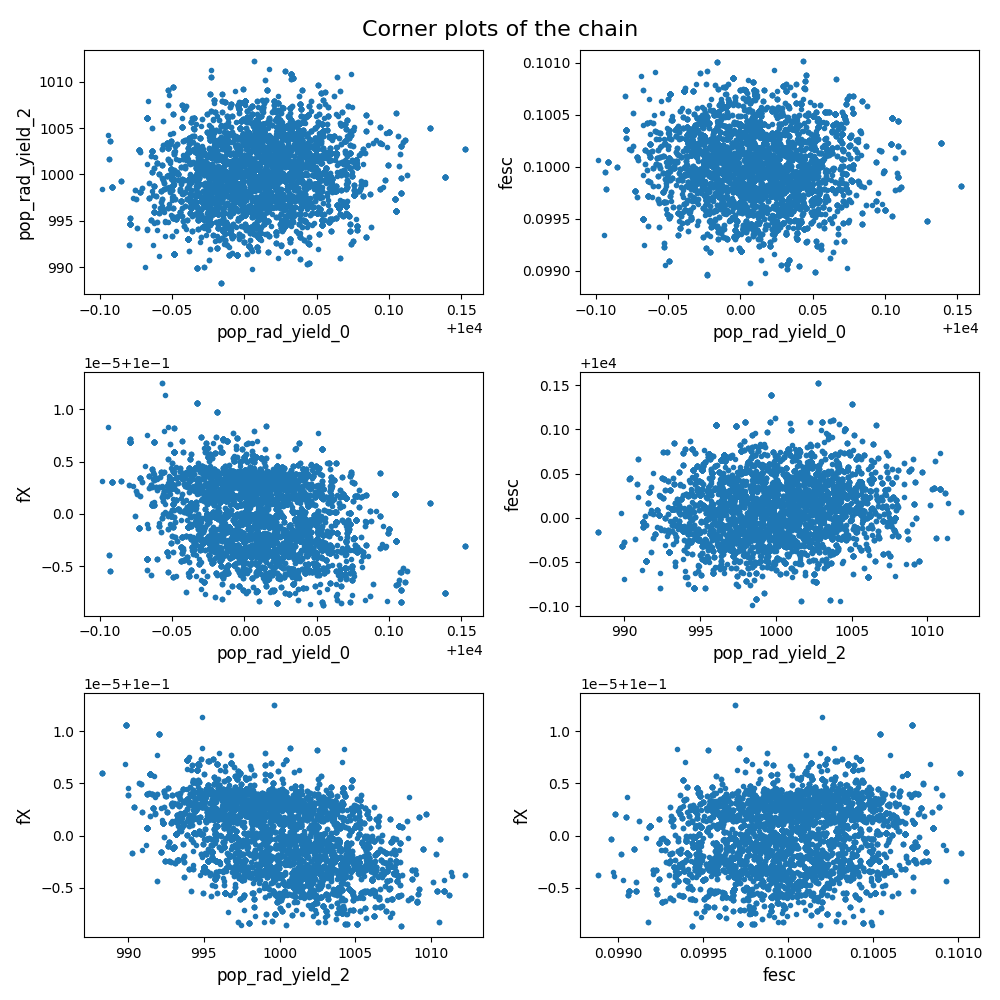
\includegraphics[scale =0.6]{corner_plots_known_curve.png}
\caption[Corner plots of the mock data chain]{Corner plots of the mock data chain indicate the correlation between the parameters. The lower left panel, which depicts the values of $f_X$ and $pop\_rad\_yield\_2$, shows the highest amount of correlation between a pair of parameters among all the six panels.}
\label{fig:corner_plots_known_curve}
\end{figure}
%@@@@@@@@@@@@@@@@@@@@@@@@@@@@@@@@@@@@@@@@@@@@@@@@@@@@@@@@@@@@@@@@@@@@@@@@@@
\begin{figure}[h!]
\centering
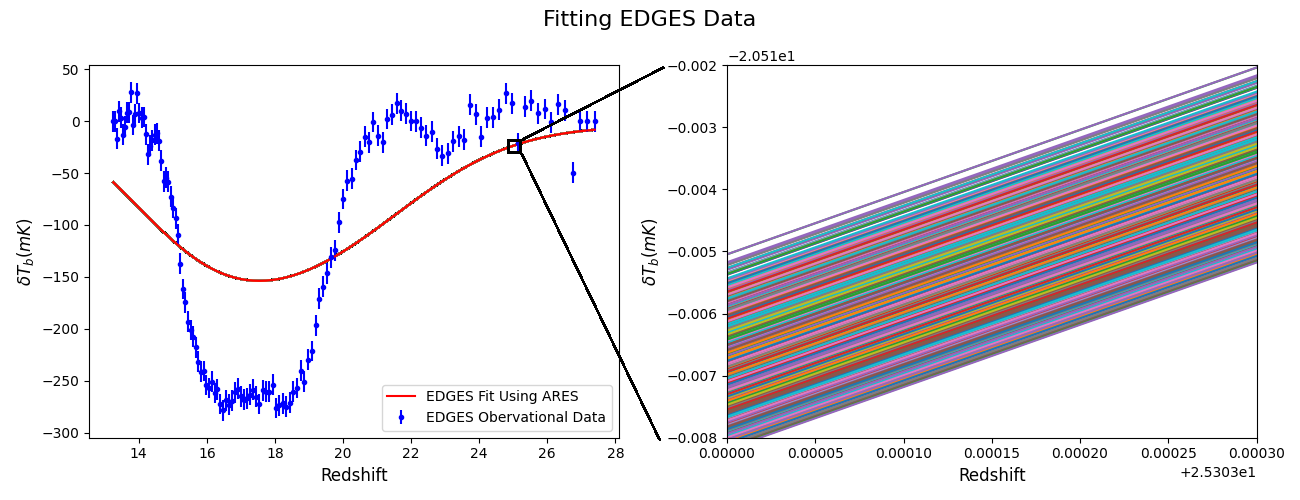
\includegraphics[scale =0.7]{fit_curve_edges.png}
\caption[Results of fitting \gls{edges} data]{Results of fitting \gls{edges} data. On the \textbf{left panel}, the blue dotted curve represents the half-amplitude \gls{edges} data and the associated uncertainty calculated using the radiometer equation ($10mK$). The red curve demonstrates the fit curve (table \ref{tab:mcmc_results_edges}). Despite using the half-amplitude data, the fit portrays a significant discrepancy with respect to the observed data, further suggesting the impossibility of achieving the \gls{edges} curve with the current well-accepted standard physics. The \textbf{right panel} is the zoomed version of the left figure, showing the two-sigma confidence interval of the fit (8780 curves), which is not visible on the left.}
\label{fig:fit_curve_edges}
\end{figure}

\begin{figure}[h!]
\centering
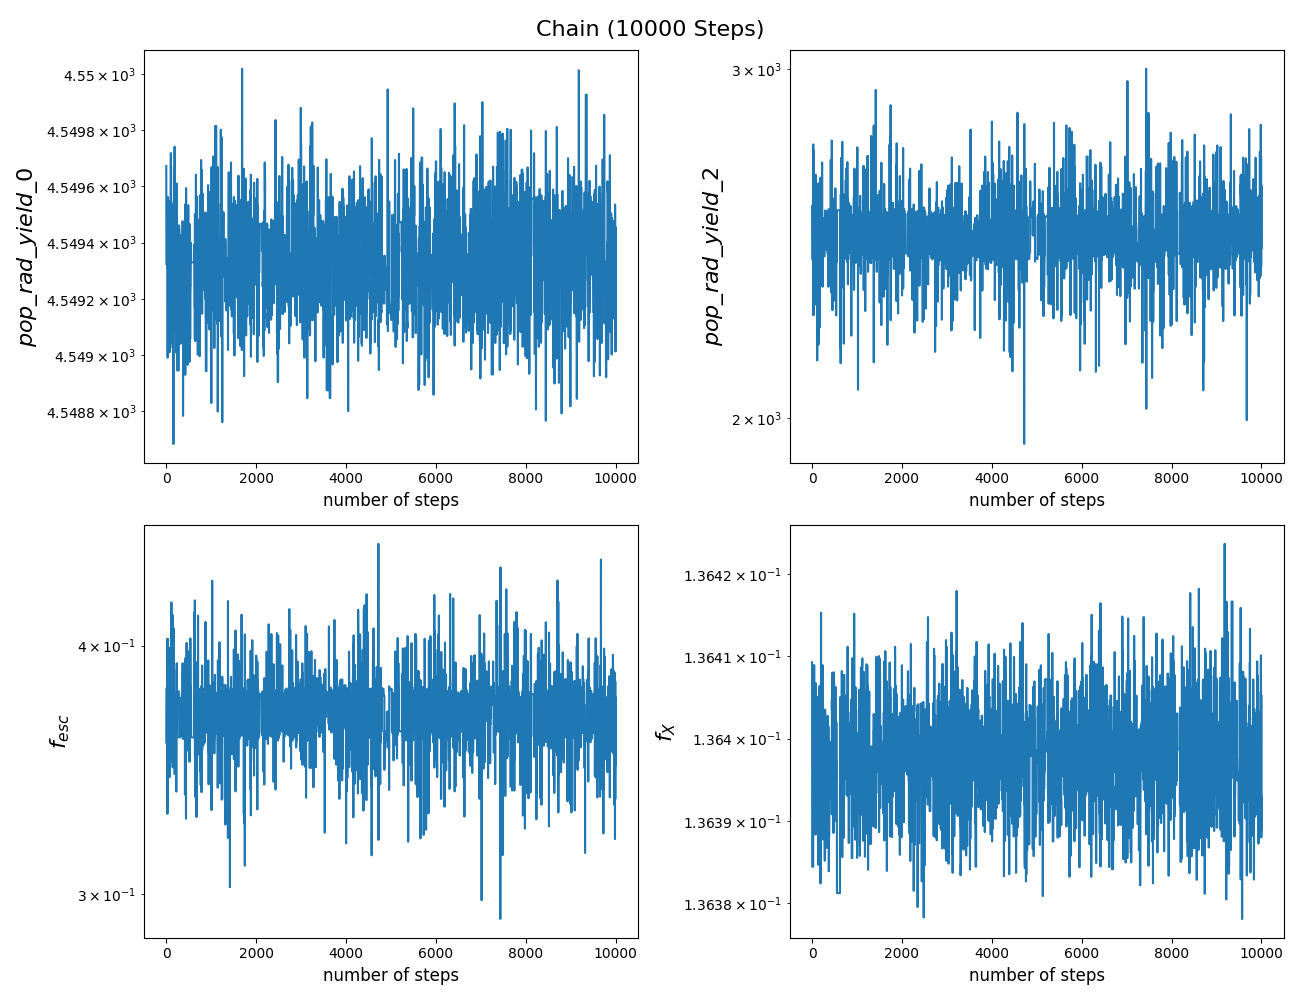
\includegraphics[scale =0.5]{chain_edges.png}
\caption[Trend of parameters in the \gls{edges} data \gls{mcmc} chain]{Trend of parameters in the $10^4$ steps \gls{mcmc} chain to fit the \gls{edges} data. The depicted white noise behavior is considered as the sign of the convergence of the \gls{mcmc} chain (refer to \ref{chap:method,sub:mcmc,subsub:convergence}). The acceptance ratio of the chain is  $23.02\%$, close to the ideal of $25\%$. The one-sigma error bar of the fit (table \ref{tab:mcmc_results_edges}) is the standard deviation of this chain.} 
\label{fig:chain_edges}
\end{figure}

\begin{figure}[h!]
\centering
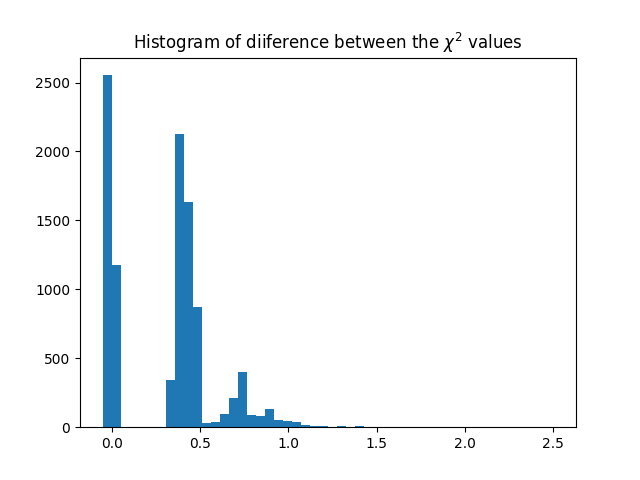
\includegraphics[scale =0.7]{csq_hist_edges.png}
\caption[Histogram of disparity in the Chi-Square of drawn samples for the \gls{EDGES} data \gls{mcmc} chain]{Histogram of disparity in the Chi-Square of drawn samples for the \gls{edges} data \gls{mcmc} chain, the mean is 0.28 with a standard deviation of 0.3. Based on the discussions of \ref{chap:method,sub:test,subsub:chi}, we expected the mean to be approximately 4.}
\label{fig:csq_hist_edges}
\end{figure}


\begin{figure}[h!]
\centering
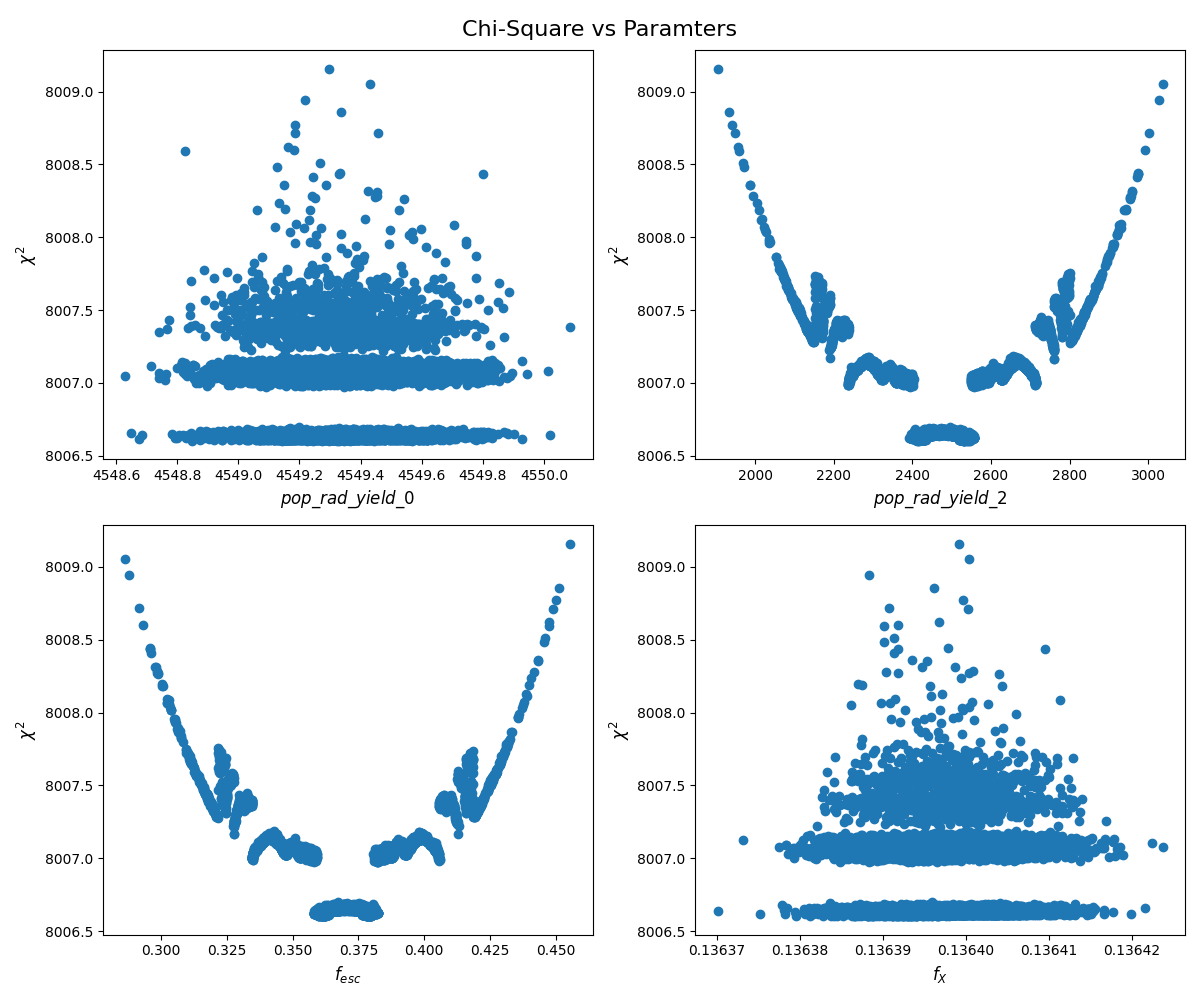
\includegraphics[scale =0.5]{csq_vs_params_edges.png}
\caption[Chi-Square of Drawn samples as a function of parameter values for \gls{edges} data]{Figures demonstrating the values of chi-square associated with the drawn samples versus the values of parameters for the \gls{edges} data set. The $\chi^2$ is expected to have a parabolic dependency on the value of parameters, which is only evident in two of the panels (upper left and lower right).}
\label{fig:csq_vs_params_edges}
\end{figure}

\begin{figure}[h!]
\centering
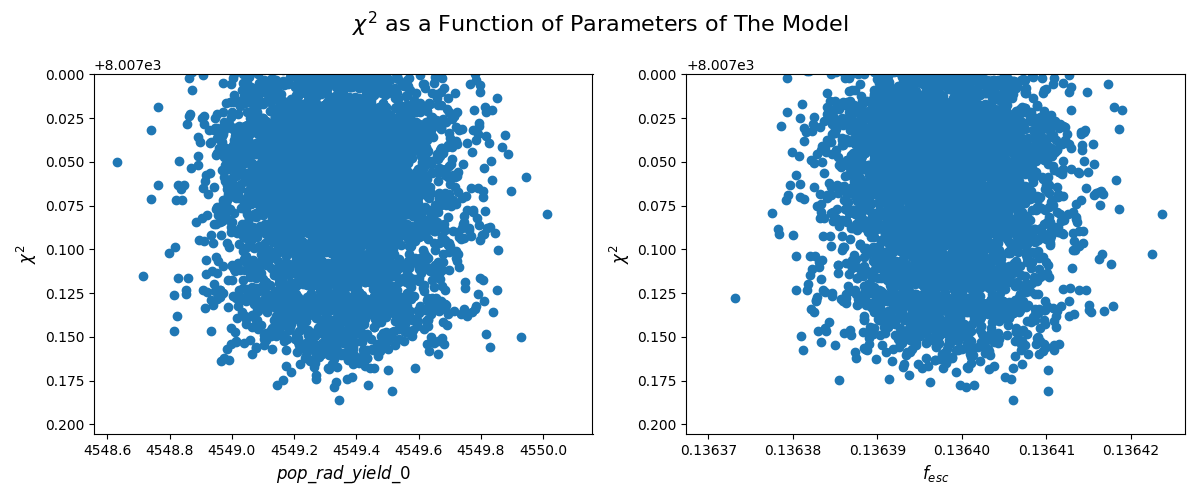
\includegraphics[scale =0.5]{csq_vs_params_zoomed_edges.png}
\caption[Chi-Square of Drawn samples as a function of parameter values for the \gls{edges} data, zoomed version]{Zoomed version of the upper left and lower right panels of Figure \ref{fig:csq_vs_params_edges}. A weak parabolic behavior is observed for low values of $\chi^2$. However, the overall shape is not completely consistent with the expectations of Figure \ref{fig:csq_params}.}
\label{fig:csq_vs_params_zoomed_edges}
\end{figure}


\begin{figure}[h!]
\centering
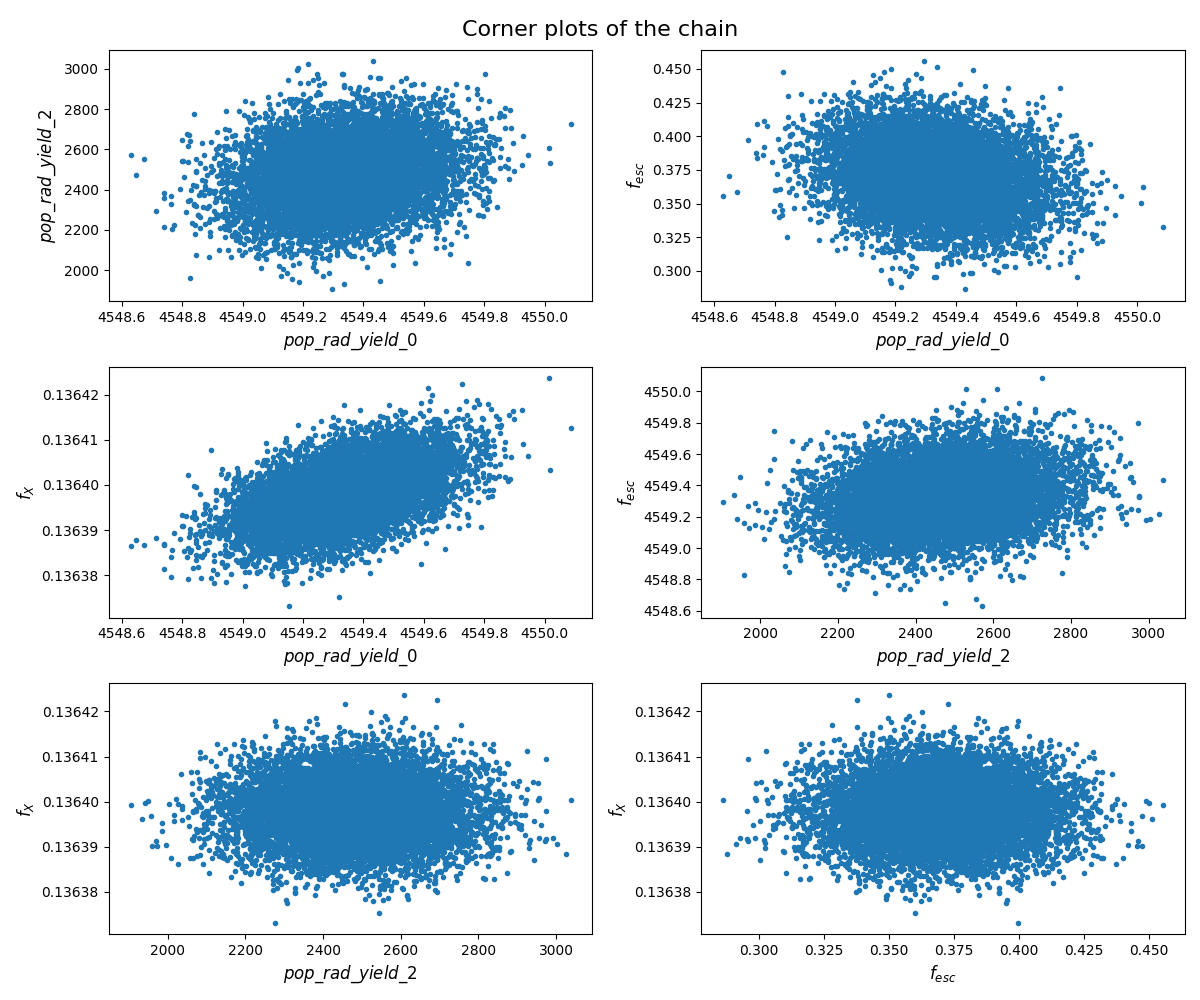
\includegraphics[scale =0.5]{corner_plots_edges.png}
\caption[Corner plots of the \gls{edges} data \gls{mcmc} chain]{Corner plots of the \gls{edges} data \gls{mcmc} chain indicate the correlation between the parameters. The middle left panel, which depicts the values of $f_X$ and $pop\_rad\_yield\_0$, appears to show the only correlation between a pair of parameters among all the six panels.}
\label{fig:corner_plots_edges}
\end{figure}
%###################################################################################
\chapter{Summary and Conclusion}
\label{chap:discussion}
Constraining the period between the dark ages and reionization has recently emerged as one of the challenges of modern radio astronomy. The motivation behind this interest is the fact that there is a clear correlation between the key features of the global $21cm$ signal and underlying astrophysical properties of the high redshift Universe (e.g., \gls{lya} intensity, the X-ray heating rate, and the production rate of ionizing photons). These correlations can be used to directly link measurements of the global $21cm$ signal to astrophysical quantities \cite{chart_param_space}.
Therefore, numerous researchers have conducted various parameter estimation methods for the data gathered from the observations focused on this signal.\par

In \cite{pe_galaxy_formation}, authors reported one of the first attempts to forecast constraints on four astrophysical parameters of interest from mock observations of the global $21cm$ signal. They especially focused on the behavior of the turning points on the global curve to constrain model parameters. Such measurements have the ability to constrain the ionization and thermal state of the \gls{igm} simultaneously. On the other hand, a combined study of the $21cm$ power spectrum and global signal measurements has the benefit of reducing the number of essential parameters needed to describe the global signal. Moreover, taking advantage of this new piece of information will result in a lower error bar on the values of cosmological parameters compared to the previously reported constraints \cite{21cmpower_global_comnbine}. \par

In an attempt to constrain astrophysical and cosmological parameters at the same time, the \emph{CosmoReionMC}, a \gls{mcmc}-based parameter estimation package, was introduced in 2021. The theoretical model of this analysis includes the effect of five cosmological and seven astrophysical parameters (related to stellar populations). Utilization of this package on \gls{edges} data showed that a short-lived population of metal-free (PopIII) stars with efficient radio emission is required to match the reported absorption amplitude. This new finding suggested an earlier reionization compared to the analysis only based on \gls{cmb} and quasar data. Although this method was successful in matching the position and depth of the \gls{edges} absorption trough, however, its abilities were limited in matching the exact shape of the signal \cite{pe_mcmc_1}.\par

Besides the traditionally well-known \gls{mcmc} approaches, \gls{ann} may also be used to extract the astrophysical parameters from the simulated and observational data sets and infer the physical state of the gas at high redshifts. This method showed particular precision in the mock data and was able to construct the magnitude of the \gls{edges} data but faced difficulties in mimicking the flattened nature of this observational signal \cite{pe_nn_1}.\par

Motivated by the findings of previous studies, in this thesis, we examined the capability of the global $21cm$ signal to assist us in our investigation of the existence of mechanisms beyond the standard model of cosmology and particle physics. The literature review provided a recap of the physics of the $21cm$ special line, its evolution through the thermal history of the universe, computational tools to simulate the global signal, and the signatures of non-standard physics. We also discussed the experimental efforts to observe this signal through the utilization of radio interferometers and the associated challenges and obstacles.\par

Knowing the fact that the global $21cm$ signal is sensitive to the underlying astrophysical processes, it is expected that the majority of the suggested non-standard scenarios would leave imprints on the value of the corresponding parameters. Therefore, we are optimistic that if such theoretical proposals exist in the early universe era, they will be revealed through parameter estimation of the existing and upcoming data. Following this idea, we introduced a parameter estimation method based on the coordinated use of \gls{lm} and \gls{mcmc}, providing a robust framework for fitting the observed data and exploring the parameter space, respectively. By employing this method, we developed a Python script specially designed for global $21cm$ applications, which takes advantage of an efficient simulator, \gls{ares}, to generate the theoretical model.\par

Finally, we presented the results of applying this method to the only claimed detection of global $21cm$ signal, the \gls{edges} data. Considering the anomalous amplitude and shape of the reported signal and the fact that the current version of our simulator \gls{ares} only contains the standard mechanisms, the output best-fit curve includes notable discrepancies with respect to the overall behavior of the empirical data. Although the developed method failed to provide us with an acceptable fit to the \gls{edges}, the process is entirely independent of the data and can be used for future released observational data sets. Furthermore, since \gls{ares} is an open-source Python module, it is possible to update the code such that it encompasses any arbitrary non-standard physics scenario. This investigation is reserved for future studies.\par

In summary, theoretical predictions of the influence of non-standard physics on global $21cm$ signal will result in the construction of a framework to decide whether the precision of prospective experiments is sufficient for observing non-standard effects.\par

\begin{comment}
The unique feature which distinguishes our study from these previous similar analyses is the employment of a simulation method solely developed for global $21cm$ applications. Therefore, we claim that our approach to estimating the astrophysical parameters of this signal is one of the most computationally-efficient methods.\par
\end{comment}

We faced certain limitations while working on this research. The majority of those are associated with the implementation of the Python script. 
A strongly limiting obstacle is related to the ARES's run-time, which is in the order of a few seconds per each simulation (approximately 4 to 5 seconds for different combinations of parameters). Given that ARES is computationally heavy, any iterative algorithm demanding to run \gls{ares} on each step is likely to require strong computational resources\footnote{ As an example, the run time for the MCMC results presented in chapter \ref{chap:results} was approximately 13 hours.}. This was the main reason that led us to combine the \gls{mcmc} with \gls{lm} in order to have a more efficient chain and guarantee its convergence.\par 

In future studies, we plan to take the analysis further and include a realistic noise model rather than an approximation. Subsequently, we shall incorporate certain non-standard effects into the \gls{ares} simulations. The same methodology will be executed to observe variations in the best-fit curve. 
The results will hopefully aid us to realize if existing and future observational data (like \gls{edges}) contain the signatures of new physics and can be explained through these proposed theories.\par

%##############################################################################

\label{chap:appendix,sub:code}
	% Begin Bibliography
	{
	
	\bibliography{references}
	\bibliographystyle{ieeetr}
	
	}
\end{document}